\documentclass[12pt, a4paper]{article}

\usepackage{amsmath}
\usepackage{amssymb}
\usepackage{booktabs}
\usepackage{ctex}
\usepackage{enumitem}
\usepackage{fancyhdr}
\usepackage{float}
\usepackage{geometry}
\usepackage{graphicx}
\usepackage[colorlinks,linkcolor=black,anchorcolor=black,citecolor=blue,CJKbookmarks=True]{hyperref}
\usepackage{listings}
\usepackage{pifont}
\usepackage{url}
\usepackage{xcolor}

\definecolor{anhao-orange}{RGB}{255,140,0}
\definecolor{anhao-purple}{RGB}{148,0,211}
\definecolor{anhao-scarlet}{RGB}{178,34,34}
\definecolor{anhao-sky}{RGB}{30,144,255}
\definecolor{anhao-background}{RGB}{230,230,250}
\geometry{left=2cm,right=2cm,top=2cm,bottom=2cm}
\renewcommand{\contentsname}{\centering{\heiti\zihao{3}{Contents}}}

\begin{document}
	
\pagenumbering{Roman}
{\tableofcontents}
\newpage

\pagenumbering{arabic}

\section{Lecture 01 - 方程组的几何解释}
\pagestyle{fancy}
\lhead{}
\chead{Lecture 01 - 方程组的几何解释}
\rhead{}

\noindent${\mathbf{n}}$ linear equations, ${\mathbf{n}}$ unknowns
\begin{itemize}
	\item row picture
	\item column picture {\textcolor{anhao-scarlet}{\bf{$\star$}}}
	\item matrix form
\end{itemize}
\vspace{14pt}
\begin{math}
\left\{  
\begin{array}{rclrcl}
	2x & - & y  & = & 0 \\
	-x & + & 2y & = & 3
\end{array}  
\right.
\end{math}
\newline
\begin{math}
\begin{bmatrix}
	2  & -1 \\
	-1 & 2
\end{bmatrix}
\begin{bmatrix}
	x \\
	y
\end{bmatrix}
=
\begin{bmatrix}
	0 \\
	3
\end{bmatrix}
\end{math}
, i.e.
\newline
${\mathbf{A}}$ (matrix of coefficients) = 
\begin{math}
\begin{bmatrix}
	2  & -1 \\
	-1 & 2
\end{bmatrix}
\end{math}
, ${\mathbf{x}}$ (vector of unknowns) = 
\begin{math}
\begin{bmatrix}
	x \\
	y
\end{bmatrix}
\end{math}
, ${\mathbf{b}}$ = 
\begin{math}
\begin{bmatrix}
	0 \\
	3
\end{bmatrix}
\end{math}
, such that
\begin{displaymath}
{\mathbf{A}}{\mathbf{x}}={\mathbf{b}}
\end{displaymath}
\vspace{14pt}
what's the {\textcolor{anhao-scarlet}{\bf{row}}} picture?
\begin{center}
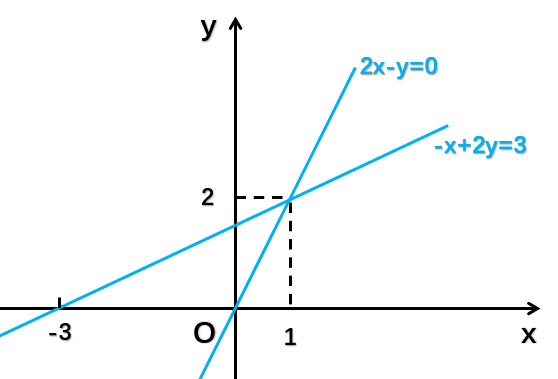
\includegraphics[width=0.4\textwidth]{figures/S1-1.png}
\end{center}
{\textcolor{anhao-purple}{to find the point that lies on both two lines}}
\newline
what's the {\textcolor{anhao-scarlet}{\bf{column}}} picture?
\newline
\begin{math}
x 
\begin{bmatrix}
	2 \\
	-1
\end{bmatrix}
+
y
\begin{bmatrix}
	-1 \\
	2
\end{bmatrix}
=
\begin{bmatrix}
	0 \\
	3
\end{bmatrix}
\end{math}
\begin{center}
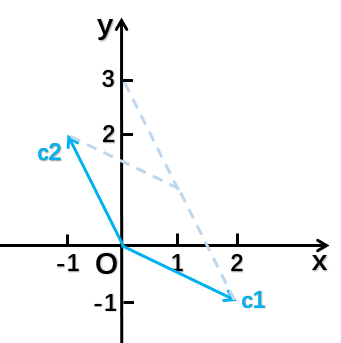
\includegraphics[width=0.3\textwidth]{figures/S1-2.png}
\end{center}
\begin{displaymath}
1{\overrightarrow{c_1}}+2{\overrightarrow{c_2}}={\overrightarrow{b}}
\end{displaymath}
{\textcolor{anhao-purple}{to find the linear combination of columns of ${\mathbf{A}}$, such that it equals ${\mathbf{b}}$}}
\vspace{14pt}
\newline
what linear combination gives ${\mathbf{b}}$?
\newline
what do all the linear combinations give?
\newline
what are all the possible, achievable right-hand sides be?
\vspace{14pt}
\newline
\begin{math}
\left\{  
\begin{array}{rclrclrclrcl}
	2x & - & y & & & = & 0 &{\bf{\textcolor{anhao-orange}{1}}}&\\
	-x & + & 2y & - & z & = & -1 &{\bf{\textcolor{anhao-orange}{2}}}&\\
	& -& 3y & + & 4z & = & 4 &{\bf{\textcolor{anhao-orange}{3}}}&
\end{array}  
\right.
\end{math}
\newline
\begin{math}
\left\{  
\begin{array}{rcl}
	&{\bf{\textcolor{anhao-orange}{1}}}&
\end{array}  
\right.
\end{math}
\quad : the plot of all the points that solve it are a plane
\newline
\begin{math}
\left\{  
\begin{array}{rcl}
	&{\bf{\textcolor{anhao-orange}{2}}}& \\
	&{\bf{\textcolor{anhao-orange}{3}}}&
\end{array}  
\right.
\end{math}
\quad : two planes meet at a line
\newline
\begin{math}
\left\{  
\begin{array}{rcl}
	&{\bf{\textcolor{anhao-orange}{1}}}& \\
	&{\bf{\textcolor{anhao-orange}{2}}}& \\
	&{\bf{\textcolor{anhao-orange}{3}}}&
\end{array}  
\right.
\end{math}
\quad : meet at a point
\newline
${\mathbf{A}}$ = 
\begin{math}
\begin{bmatrix}
	2  & -1 & 0 \\
	-1 & 2 & -1 \\
	0 & -3 & 4
\end{bmatrix}
\end{math}
, ${\mathbf{b}}$ =
\begin{math} 
\begin{bmatrix}
	0 \\
	-1\\
	4
\end{bmatrix}
\end{math}
\vspace{14pt}
\newline
what's the {\textcolor{anhao-scarlet}{\bf{row}}} picture?
\newline
{\textcolor{anhao-purple}{to find out all the points that satisfy all the equations}}
\newline
what's the {\textcolor{anhao-scarlet}{\bf{column}}} picture?
\newline
\begin{math}
x
\begin{bmatrix}
	2 \\
	-1\\
	0
\end{bmatrix}
 + y
\begin{bmatrix}
	-1 \\
	2\\
	-3
\end{bmatrix}
 + z
\begin{bmatrix}
	0 \\
	-1\\
	4
\end{bmatrix}
 = 
\begin{bmatrix}
	0 \\
	-1\\
	4
\end{bmatrix}
\end{math}
\vspace{14pt}
\newline
can I always solve ${\mathbf{A}}$${\mathbf{x}}$ = ${\mathbf{b}}$ for every right-hand side ${\mathbf{b}}$?
\newline
do the linear combinations of the columns fill 3-dimensional space?
\newline
{\textcolor{anhao-purple}{for this ${\mathbf{A}}$, the answer is {\bf{YES}} (non-singular, invertible)}}
\newline
{\textcolor{anhao-purple}{but for some others ${\mathbf{A}}$, the answer could be {\bf{NO}} (singular, not-invertible)}}
\vspace{14pt}
\newline
if the 3 columns all lie in the same plane, 
\newline
so I could solve it for some right-hand sides, when ${\overrightarrow{b}}$ is in the plane,
\newline
but most right-hand sides would be out of the plane and unreachable.
\vspace{14pt}
\newline
in some case, the combinations of ${\mathbf{n}}$ columns can only fill out ${\mathbf{m}}$-D ($m < n$)
\vspace{14pt}
\newline
\begin{math}
\begin{bmatrix}
	2 & 5 \\
	1 & 3 
\end{bmatrix}
\begin{bmatrix}
	1 \\
	2 
\end{bmatrix}
 = 
1
\begin{bmatrix}
	2 \\
	1 
\end{bmatrix}
 + 
2
\begin{bmatrix}
	5 \\
	3 
\end{bmatrix}
 = 
\begin{bmatrix}
	12 \\
	7 
\end{bmatrix}
\end{math}
\newline
${\mathbf{A}}$${\mathbf{x}}$ means: ${\mathbf{A}}$${\mathbf{x}}$ is a combination of columns of ${\mathbf{A}}$

\newpage
\section{Lecture 02 - 矩阵消元}
\pagestyle{fancy}
\lhead{}
\chead{Lecture 02 - 矩阵消元}
\rhead{}

\noindent when solving equations-system, 
\newline
{\bf{Elimination}}, if it succeeds, it gets the answer.
\newline
It's always good to ask how could it fail.
\vspace{14pt}
\newline
\begin{math}
	\left\{  
	\begin{array}{rclrclrcl}
		x & + & 2y & + & z & = & 2 \\
		3x & + & 8y & + & z & = & 12 \\
		& & 4y & + & z & = & 2 
	\end{array}  
	\right.
\end{math}
\vspace{14pt}
\newline
\begin{math}
	\begin{bmatrix}
		{\bf{\textcolor{anhao-sky}{\mathop{1}\limits_{first-pivot}}}} & 2 & 1 \\
		3 & 8 & 1 \\
		0 & 4 & 1
	\end{bmatrix}
	\xrightarrow[row_3 - 0 \times row_1]{row_2 - 3 \times row_1}
	\begin{bmatrix}
		1 & 2 & 1 \\
		0 & {\bf{\textcolor{anhao-sky}{\mathop{2}\limits_{second-pivot}}}} & -2 \\
		0 & 4 & 1
	\end{bmatrix}
	\xrightarrow[]{row_3 - 2 \times row_2}
	\begin{bmatrix}
		1 & 2 & 1 \\
		0 & 2 & -2 \\
		0 & 0 & {\bf{\textcolor{anhao-sky}{\mathop{5}\limits_{third-pivot}}}}
	\end{bmatrix}
\end{math}
\newline
{\textcolor{anhao-scarlet}{pivots can {\bf{NOT}} be 0 !}}
\newline
if there is a 0 in the pivot position, then try to switch lines
\newline
if 0 is in the pivot position and no place to exchange, then failure
\vspace{14pt}
\newline
let's bring the right-hand side in (Augmented Matrix)
\newline
\begin{math}
	\left[
	\begin{array}{ccc|c}
		1 & 2 & 1 & 2 \\
		3 & 8 & 1 & 12 \\
		0 & 4 & 1 & 2
	\end{array}
	\right]
	\longrightarrow
	\left[
	\begin{array}{ccc|c}
		1 & 2 & 1 & 2 \\
		0 & 2 & -2 & 6 \\
		0 & 4 & 1 & 2
	\end{array}
	\right]
	\longrightarrow
	\left[
	\begin{array}{ccc|c}
		1 & 2 & 1 & 2 \\
		0 & 2 & -2 & 6 \\
		0 & 0 & 5 & -10
	\end{array}
	\right]
	\Rightarrow
	\left\{  
	\begin{array}{rclrclrcl}
		x & + & 2y & + & z  & = & 2 \\
		  &   & 2y & - & 2z & = & 6  \\
		  &   &    &   & 5z & = & -10  
	\end{array}  
	\right.
\end{math}
\newline
by back-substitution: 
\begin{math}
	x = 2, y = 1, z = -2
\end{math}
\vspace{14pt}
\newline
{\bf{"elimination matrices"}}
\vspace{14pt}
\newline
\begin{math}
	\begin{bmatrix}
		{\textcolor{anhao-orange}{\vdots}} & {\textcolor{green}{\vdots}} & {\textcolor{purple}{\vdots}} \\
		{\textcolor{anhao-orange}{col_1}} & {\textcolor{green}{col_2}} & {\textcolor{purple}{col_3}} \\
		{\textcolor{anhao-orange}{\vdots}} & {\textcolor{green}{\vdots}} & {\textcolor{purple}{\vdots}}
	\end{bmatrix}
	\begin{bmatrix}
		1 \\
		2 \\
		3
	\end{bmatrix}
	 = 
	\begin{bmatrix}
		\ \\
		\ \\
		\ 
	\end{bmatrix}
	 = 
	1 \times {\textcolor{anhao-orange}{col_1}} + 2 \times {\textcolor{green}{col_2}} + 3 \times {\textcolor{purple}{col_3}}
\end{math}
\newline
{\textcolor{anhao-purple}{the result of multiplying a matrix by some vectors, is a combination of columns of the matrix}}
\vspace{14pt}
\newline
\begin{math}
	\begin{bmatrix}
		1 & 2 & 7
	\end{bmatrix}
	\begin{bmatrix}
		{\textcolor{anhao-orange}{\cdots}} & {\textcolor{anhao-orange}{row_1}} & {\textcolor{anhao-orange}{\cdots}} \\
		{\textcolor{green}{\cdots}} & {\textcolor{green}{row_2}} & {\textcolor{green}{\cdots}} \\
		{\textcolor{purple}{\cdots}} & {\textcolor{purple}{row_3}} & {\textcolor{purple}{\cdots}}
	\end{bmatrix}
	 = 
	\begin{bmatrix}
		\ & \ & \
	\end{bmatrix}
	 = 
	\begin{array}{rcl}
		1 & \times &  {\textcolor{anhao-orange}{row_1}} \\
		 & + & \\
		2 & \times & {\textcolor{green}{row_2}} \\
		 & + & \\
		7 & \times & {\textcolor{purple}{row_3}}
	\end{array}
\end{math}
\newline
{\textcolor{anhao-purple}{the product of a row times a matrix, is a combination of rows of the matrix}}
\vspace{14pt}
\newline
when we do matrix multiplication, keep your eye on what it is doing with the whole vectors
\vspace{14pt}
\newline
what does the matrix, which can subtract $3 \times row_1$ from $row_2$ look like?
\newline
i.e. 
\begin{math}
	\begin{bmatrix}
		? & ? & ? \\
		? & ? & ? \\
		? & ? & ? 
	\end{bmatrix}
	\begin{bmatrix}
		1 & 2 & 1 \\
		3 & 8 & 1 \\
		0 & 4 & 1 
	\end{bmatrix}
	 = 
	\begin{bmatrix}
		1 & 2 & 1 \\
		0 & 2 & -2 \\
		0 & 4 & 1 
	\end{bmatrix}
\end{math}
\newline
\begin{math}
	\begin{bmatrix}
		? & ? & ? \\
		? & ? & ? \\
		? & ? & ? 
	\end{bmatrix}
	\\
	\xrightarrow[]{as \ R_1 = {\textcolor{anhao-scarlet}{\bf{1}}} \times row_1 + {\textcolor{anhao-scarlet}{\bf{0}}} \times row_2 + {\textcolor{anhao-scarlet}{\bf{0}}} \times row_3}
	\begin{bmatrix}
		1 & 0 & 0 \\
		? & ? & ? \\
		? & ? & ? 
	\end{bmatrix}
	\\
	\xrightarrow[]{as \ R_3 = {\textcolor{anhao-scarlet}{\bf{0}}} \times row_1 + {\textcolor{anhao-scarlet}{\bf{0}}} \times row_2 + {\textcolor{anhao-scarlet}{\bf{1}}} \times row_3}
	\begin{bmatrix}
		1 & 0 & 0 \\
		? & ? & ? \\
		0 & 0 & 1 
	\end{bmatrix}
	\\
	\xrightarrow[]{as \ R_2 = {\textcolor{anhao-scarlet}{\bf{-3}}} \times row_1 + {\textcolor{anhao-scarlet}{\bf{1}}} \times row_2 + {\textcolor{anhao-scarlet}{\bf{0}}} \times row_3}
	\begin{bmatrix}
		1 & 0 & 0 \\
		-3 & 1 & 0 \\
		0 & 0 & 1 
	\end{bmatrix}
\end{math}
\newline
\begin{math}
	\begin{bmatrix}
		1 & 0 & 0 \\
		-3 & 1 & 0 \\
		0 & 0 & 1 
	\end{bmatrix}
\end{math}
: elementary matrix (初等矩阵)
\newline
${\mathbf{E_{i,j}}}$ means it's the matrix that we use to fix the (i, j) position
\newline
e.g. 
\begin{math}
	\begin{bmatrix}
		? & ? & ? \\
		? & ? & ? \\
		? & ? & ? 
	\end{bmatrix}
	\xrightarrow[]{R_1=row_1}
	\begin{bmatrix}
		1 & 0 & 0 \\
		? & ? & ? \\
		? & ? & ? 
	\end{bmatrix}
	\xrightarrow[]{R_2=row_2}
	\begin{bmatrix}
		1 & 0 & 0 \\
		0 & 1 & 0 \\
		? & ? & ? 
	\end{bmatrix}
	\xrightarrow[]{R_3 = row_3 - 2 \times row_2}
	\begin{bmatrix}
		1 & 0 & 0 \\
		0 & 1 & 0 \\
		0 & -2 & 1 
	\end{bmatrix}
	 = 
	E_{3,2}
\end{math}
\vspace{14pt}
\newline
in elimination, we can use an elementary matrix to describe the change in each step
\vspace{14pt}
\newline
the next point in this lecture is to put these steps together, into a matrix that does these steps all in sequence, in another words, how could I create the matrix that does the whole job at once? i.e.
\begin{displaymath}
	{\mathbf{E_{3,2}}}({\mathbf{E_{2,1}}}{\mathbf{A}}) = {\mathbf{U}} \Longleftrightarrow {\mathbf{\boxed{?}}}{\mathbf{A}} = {\mathbf{U}}
\end{displaymath}
\vspace{14pt}
\newline
{\bf{Associative Law}}
\begin{displaymath}
	({\mathbf{A}}{\mathbf{B}}){\mathbf{C}} = {\mathbf{A}}({\mathbf{B}}{\mathbf{C}})
\end{displaymath}
\vspace{14pt}
\newline
permutation(置换): 
\begin{itemize}
	\item exchange rows, e.g.
	\par 
	\begin{math}
		\begin{bmatrix}
			? & ? \\
			? & ?
		\end{bmatrix}
		\begin{bmatrix}
			a & b \\
			c & d
		\end{bmatrix}
		 = 
		\begin{bmatrix}
			c & d \\
			a & b
		\end{bmatrix}
	\end{math}
	\par ${\mathbf{P}}$ = 
	\begin{math}
		\begin{bmatrix}
			0 & 1 \\
			1 & 0
		\end{bmatrix}
	\end{math}
	is to exchange $row_1$ and $row_2$
	\item exchange columns, e.g.
	\par 
	\begin{math}
		\begin{bmatrix}
			a & b \\
			c & d
		\end{bmatrix}
		\begin{bmatrix}
			? & ? \\
			? & ?
		\end{bmatrix}
		= 
		\begin{bmatrix}
			b & a \\
			d & c
		\end{bmatrix}
	\end{math}
	\par ${\mathbf{P}}$ = 
	\begin{math}
		\begin{bmatrix}
			0 & 1 \\
			1 & 0
		\end{bmatrix}
	\end{math}
	is to exchange $col_1$ and $col_2$
\end{itemize}
\vspace{14pt}
{\textcolor{anhao-purple}{when I multiply a matrix on the left, I am doing row operations}}
\newline
{\textcolor{anhao-purple}{if I want to do column operations, I should put a matrix on the right}}
\vspace{14pt}
\newline
if ${\mathbf{\boxed{?}}}{\mathbf{A}} = {\mathbf{U}}$, then how can I "from ${\mathbf{U}}$ back to ${\mathbf{A}}$"?
\newline
this is about reversing steps, invertible, $\cdots$
\newline
\begin{math}
	\begin{bmatrix}
		1 & 0 & 0 \\
		-3 & 1 & 0 \\
		0 & 0 & 1
	\end{bmatrix}^{-1}
	 = 
	\begin{bmatrix}
		1 & 0 & 0 \\
		3 & 1 & 0 \\
		0 & 0 & 1
	\end{bmatrix}
\end{math}
\newline
"what steps can get me back?"
\newline
"what matrix can bring me back?"

\newpage
\section{Lecture 03 - 乘法和逆矩阵}
\pagestyle{fancy}
\lhead{}
\chead{Lecture 03 - 乘法和逆矩阵}
\rhead{}

\noindent
key words:
\begin{itemize}
	\item matrix multiplication (4 ways)
	\item inverse of ${\mathbf{A}}$, ${\mathbf{AB}}$, ${\mathbf{A^{T}}}$
	\item Gauss-Jordan, to find ${\mathbf{A^{-1}}}$
\end{itemize}
\vspace{14pt}
\begin{math}
	\underbrace{
		\begin{bmatrix}
			\ \ & \ & \ & \ \ \\
			\ \ & \ & \ & \ \ \\
			\ \ & \ & \ & \ \ 
		\end{bmatrix}
	}_{\mathbf{A}}
	\underbrace{
		\begin{bmatrix}
			\ \ & \ & \ \ \\
			\ \ & \ & \ \ \\
			\ \ & \ & \ \ \\
			\ \ & \ & \ \ 
		\end{bmatrix}
	}_{\mathbf{B}}
	 = 
	\underbrace{
		\begin{bmatrix}
			\ \ & \ & \ \ \\
			\ \ & c_{i,j} & \ \ \\
			\ \ & \ & \ \ 
		\end{bmatrix}
	}_{\mathbf{C=AB}}
\end{math}
\newline
$c_{i,j}$ comes from $row_i$ of ${\mathbf{A}}$ and $col_j$ of ${\mathbf{B}}$
\newline
e.g.
\par 
\begin{math}
	\begin{aligned}
		c_{3,4} &= 
		\begin{bmatrix}
			\ & \ & \ & \ & \ \\
			\ & {\textcolor{anhao-orange}{row_3}} & {\textcolor{anhao-orange}{of}} & {\textcolor{anhao-orange}{\mathbf{A}}} & \ \\
			\ & \ & \ & \ & \ 
		\end{bmatrix}
		\begin{bmatrix}
			\ & \ & \ \\
			\ & {\textcolor{anhao-purple}{col_4}} & \ \\
			\ & {\textcolor{anhao-purple}{of}} & \ \\
			\ & {\textcolor{anhao-purple}{\mathbf{B}}} & \ \\
			\ & \ & \
		\end{bmatrix} \\
				&= a_{3,1}b_{1,4} + a_{3,2}b_{2,4} + \cdots + a_{3,i}b_{i,4} + \cdots + a_{3,n}b_{n,4} \\
				&= \sum_{k=1}^{n}a_{3,k}b_{k,4}
	\end{aligned}
\end{math}
\vspace{14pt}
\newline
{\textcolor{anhao-scarlet}{the number of columns of ${\mathbf{A}}$ has to match the number of rows of ${\mathbf{B}}$}
\begin{displaymath}
	{\mathbf{A}}_{m \times n}{\mathbf{B}}_{n \times p} = {\mathbf{C}}_{m \times p}
\end{displaymath}
\vspace{14pt}
the matrix times the $n^{\text{th}}$ column is the $n^{\text{th}}$ column of the answer
\begin{center}
	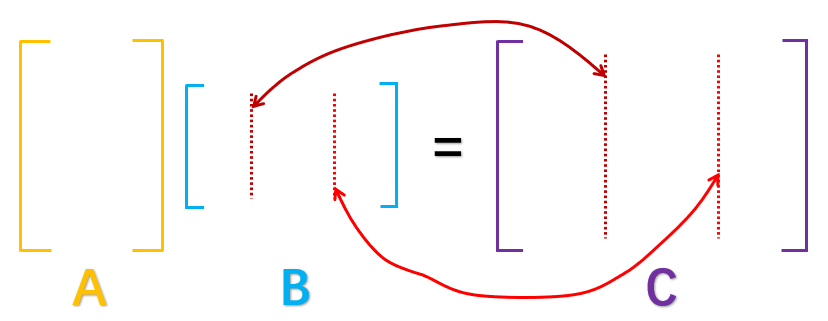
\includegraphics[scale=0.5]{figures/S3-1.png}
\end{center}
so I could think of multiplying a matrix by a vector, side by side
\newline
I can just think of having several columns, multiplying by ${\mathbf{A}}$, and getting the columns of answer
\vspace{14pt}
\newline
{\textcolor{anhao-purple}{the columns of ${\mathbf{C}}$ are combinations of columns of ${\mathbf{A}}$}}
\newline
$\Longleftrightarrow$ every column of ${\mathbf{C}}$ is a combination of columns of ${\mathbf{A}}$, and numbers in ${\mathbf{B}}$ tell me what the combination is
\newline
in the same way, {\textcolor{anhao-purple}{the rows of ${\mathbf{C}}$ are combinations of rows of ${\mathbf{B}}$}}
\vspace{14pt}
\newline
what about " 
\begin{math}
	\underbrace{col \ \ of \ \ {\mathbf{A}}}_{m \times 1}
	\quad \times \quad
	\underbrace{row \ \ of \ \ {\mathbf{B}}}_{1 \times p}
\end{math}
 "?
\newline
e.g.
\par 
\begin{math}
	\begin{bmatrix}
		2 \\
		3 \\
		4
	\end{bmatrix}
	\begin{bmatrix}
		1 & 6
	\end{bmatrix}
	 = 
	\begin{bmatrix}
		2 & 12 \\
		3 & 18 \\
		4 & 24 
	\end{bmatrix}
\end{math}
\par 
\begin{math}
	\begin{bmatrix}
		2 & 7 \\
		3 & 8 \\
		4 & 9 
	\end{bmatrix}
	\begin{bmatrix}
		1 & 6 \\
		0 & 0 
	\end{bmatrix}
	 = 
	\begin{bmatrix}
		2 \\
		3 \\
		4
	\end{bmatrix}
	\begin{bmatrix}
		1 & 6
	\end{bmatrix}
	 + 
	\begin{bmatrix}
		7 \\
		8 \\
		9
	\end{bmatrix}
	\begin{bmatrix}
		0 & 0
	\end{bmatrix}
\end{math}
\newline
\begin{math}
	\begin{aligned}
		{\mathbf{AB}} &= {\text{sum of}} \ \ (col_i \ of \ {\mathbf{A}}) \times (row_i \ of \ {\mathbf{B}}) \\
		&= \sum_{i=1}^{n}(col_i \ of \ {\mathbf{A}}) \times (row_i \ of \ {\mathbf{B}})
	\end{aligned}
\end{math}
\vspace{14pt}
\newline
{\textcolor{anhao-purple}{the row space}} for 
\begin{math}
	\begin{bmatrix}
		2 & 12 \\
		3 & 18 \\
		4 & 24
	\end{bmatrix}
\end{math}
, which is like all combinations of the rows, is the line through the row-vector 
\begin{math}
	\begin{bmatrix}
		1 & 6
	\end{bmatrix}
\end{math}, the same to {\textcolor{anhao-purple}{the column space}}
\vspace{14pt}
\newline
you could also cut the matrix into blocks and do the multiplication by blocks, i.e.
\begin{displaymath}
	\underbrace{
		\left[
		\begin{array}{c|c}
			{\mathbf{A_1}} & {\mathbf{A_2}} \\
			\hline
			{\mathbf{A_3}} & {\mathbf{A_4}}
		\end{array}
		\right]
	}_{{\mathbf{A}}}
	\underbrace{
		\left[
		\begin{array}{c|c}
			{\mathbf{B_1}} & {\mathbf{B_2}} \\
			\hline
			{\mathbf{B_3}} & {\mathbf{B_4}}
		\end{array}
		\right]
	}_{{\mathbf{B}}}
	 = 
	\underbrace{
		\left[
		\begin{array}{c|c}
			{\mathbf{A_1B_1+A_2B_3}} & {\mathbf{A_1B_2+A_2B_4}} \\
			\hline
			{\mathbf{A_3B_1+A_4B_3}} & {\mathbf{A_3B_2+A_4B_4}}
		\end{array}
		\right]
	}_{{\mathbf{AB}}}
\end{displaymath}
\vspace{14pt}
\newline
\noindent{\textcolor{anhao-purple}{Inverses (square matrices)}}
\newline
not all matrices have inverses, if a matrix is square, is it invertible or not?
\newline
if ${\mathbf{A}}$ is invertible, non-singular, then
\begin{displaymath}
	{\mathbf{A^{-1}}}{\mathbf{A}} = {\mathbf{I}} = {\mathbf{A}}{\mathbf{A^{-1}}}
\end{displaymath}
in singular case, no inverse!
\newline
e.g.
\par 
\begin{math}
	{\mathbf{A}} = 
	\begin{bmatrix}
		1 & 3 \\
		2 & 6
	\end{bmatrix}
\end{math}
\par thinking about columns here, if I multiply ${\mathbf{A}}$ by some other matrices, the columns of the results are all multiples of 
\begin{math}
	\begin{bmatrix}
		1 \\
		2
	\end{bmatrix}
\end{math}
, so no way to get the identity matrix ${\mathbf{I}}$
\par there is another more important reason
\par a square matrix has no inverse if I can find a vector ${\mathbf{x}}$ such that ${\mathbf{A}}{\mathbf{x}} = {\mathbf{0}}$ and ${\mathbf{x}} \neq {\mathbf{0}}$
\par but 
\par \qquad
\begin{math}
	\begin{bmatrix}
		1 & 3 \\
		2 & 6
	\end{bmatrix}
	\begin{bmatrix}
		3 \\
		-1
	\end{bmatrix}
	 = 
	\begin{bmatrix}
		0 \\
		0
	\end{bmatrix}
\end{math}
\vspace{14pt}
\newline
{\textcolor{anhao-scarlet}{the matrix can't have an inverse if some columns give no contribution!}}
\vspace{14pt}
\newline
because
\par if 
\begin{math}
	{\mathbf{A}} = 
	\begin{bmatrix}
		1 & 3 \\
		2 & 6
	\end{bmatrix}
\end{math}
 has an inverse, named ${\mathbf{A^{-1}}}$, then 
\begin{math}
	{\mathbf{A^{-1}}}{\mathbf{A}}
	\begin{bmatrix}
		3 \\
		-1
	\end{bmatrix}
	 = 
	{\mathbf{A^{-1}}}
	\begin{bmatrix}
		0 \\
		0
	\end{bmatrix}
\end{math}
, 
\par 
and meanwhile, 
\begin{math}
	{\mathbf{A^{-1}}}{\mathbf{A}}
	\begin{bmatrix}
		3 \\
		-1
	\end{bmatrix}
	= 
	{\mathbf{I}}
	\begin{bmatrix}
		3 \\
		-1
	\end{bmatrix}
	 = 
	\begin{bmatrix}
		3 \\
		-1
	\end{bmatrix}
\end{math}
, 
\par
so that 
\begin{math}
	\begin{bmatrix}
		3 \\
		-1
	\end{bmatrix}
	 = 
	\begin{bmatrix}
		0 \\
		0
	\end{bmatrix}
\end{math}
, which is not True
\vspace{14pt}
\newline
{\textcolor{anhao-scarlet}{our conclusion is that for non-invertible/singular matrices, some combinations of their columns give the zero column}}
\vspace{14pt}
\newline
let's take a matrix that does have an inverse for example
\newline
e.g.
\par 
\begin{math}
	{
		\underbrace{
			\begin{bmatrix}
				1 & 3 \\
				2 & 7
			\end{bmatrix}
		}_{\mathbf{A}}
	}
	{
		\underbrace{
			\begin{bmatrix}
				a & b \\
				c & d
			\end{bmatrix}
		}_{\mathbf{A^{-1}}}
	}
	 = 
	{
		\underbrace{
			\begin{bmatrix}
				1 & 0 \\
				0 & 1
			\end{bmatrix}
		}_{\mathbf{I}}
	}
\end{math}
\par then
\begin{math}
	\left\{  
	\begin{array}{rcl}
		{\mathbf{A}}
		\begin{bmatrix}
			a \\
			b 
		\end{bmatrix}
		& = & 
		\begin{bmatrix}
		 	1 \\
		 	0 
		\end{bmatrix} 
		\\
		{\mathbf{A}}
		\begin{bmatrix}
			c \\
			d 
		\end{bmatrix}
		& = & 
		\begin{bmatrix}
		 	0 \\
		 	1 
		\end{bmatrix}
	\end{array}  
	\right.
\end{math}
\newline
generally, 
\begin{displaymath}
	{\mathbf{A}} \cdot (col_j \ of \ {\mathbf{A^{-1}}}) = (col_j \ of \ {\mathbf{I}})
\end{displaymath}
\vspace{14pt}
\newline
then how to solve the inverse for an invertible matrix?
\newline
here is the Gauss-Jordan idea, to solve two equations at once
\newline
\begin{math}
	\left\{  
	\begin{array}{rcl}
		\begin{bmatrix}
			1 & 3 \\
			2 & 7 
		\end{bmatrix}
		\begin{bmatrix}
			a \\
			b 
		\end{bmatrix}
		& = & 
		\begin{bmatrix}
			1 \\
			0 
		\end{bmatrix} 
		\\
		\begin{bmatrix}
			1 & 3 \\
			2 & 7 
		\end{bmatrix}
		\begin{bmatrix}
			c \\
			d 
		\end{bmatrix}
		& = & 
		\begin{bmatrix}
			0 \\
			1 
		\end{bmatrix}
	\end{array}  
	\right.
\end{math}
\newline
"solve them together!"
\newline
\begin{math}
	\underbrace{
		\left[
		\begin{array}{cc|cc}
			1 & 3 & 1 & 0 \\
			2 & 7 & 0 & 1
		\end{array}
		\right]
	}_{
		\left[
		\begin{array}{c|c}
			{\mathbf{A}} & {\mathbf{I}}
		\end{array}
		\right]
	}
	\rightarrow
	\left[
	\begin{array}{cc|cc}
		1 & 3 & 1 & 0 \\
		0 & 1 & -2 & 1
	\end{array}
	\right]
	\rightarrow
	\underbrace{
		\left[
		\begin{array}{cc|cc}
			1 & 0 & 7 & -3 \\
			0 & 1 & -2 & 1
		\end{array}
		\right]
	}_{
		\left[
		\begin{array}{c|c}
			{\mathbf{I}} & {\mathbf{A^{-1}}}
		\end{array}
		\right]
	}
\end{math}
\newline
把单位矩阵当成草稿纸,记录下对左侧矩阵的变换
\newline
相当于左右两边同时乘上逆矩阵,当左边变成单位矩阵时,右边即是该逆矩阵
\newline
i.e.
\par
\begin{math}
	\begin{aligned}
		{\mathbf{E}}_{i_1,j_1}
		{\mathbf{E}}_{i_2,j_2}
		\cdots
		{\mathbf{E}}_{i_n,j_n}
		\left[
		\begin{array}{c|c}
			{\mathbf{A}} & {\mathbf{I}}
		\end{array}
		\right]
		&= 
		\left[
		\begin{array}{c|c}
			{{\mathbf{E}}_{i_1,j_1}{\mathbf{E}}_{i_2,j_2}\cdots{\mathbf{E}}_{i_n,j_n}{\mathbf{A}}} & {{\mathbf{E}}_{i_1,j_1}{\mathbf{E}}_{i_2,j_2}\cdots{\mathbf{E}}_{i_n,j_n}{\mathbf{I}}}
		\end{array}
		\right]
		\\
		&= 
		\left[
		\begin{array}{c|c}
			{\mathbf{I}} & 
			{\mathbf{E}}_{i_1,j_1}{\mathbf{E}}_{i_2,j_2}\cdots{\mathbf{E}}_{i_n,j_n}
		\end{array}
		\right]
	\end{aligned}
\end{math}
\par
then 
\begin{math}
	{\mathbf{A^{-1}}} = {\mathbf{E}}_{i_1,j_1}{\mathbf{E}}_{i_2,j_2}\cdots{\mathbf{E}}_{i_n,j_n}
\end{math}
\par 注:
\par\qquad 
\begin{math}
	{\mathbf{E}}_{i_t,j_t}
	\left[
	\begin{array}{c|c}
		{\mathbf{A}} & {\mathbf{I}}
	\end{array}
	\right]
\end{math}
,即对
\begin{math}
	\left[
	\begin{array}{c|c}
		{\mathbf{A}} & {\mathbf{I}}
	\end{array}
	\right]
\end{math}
做行变换
$\Longleftrightarrow$
对${\mathbf{A}}$与${\mathbf{I}}$同时、做同样的行变换
\par\qquad 
同理,可以对
\begin{math}
	\left[
	\begin{array}{c}
		{\mathbf{A}} \\
		\hline
	    {\mathbf{I}}
	\end{array}
	\right]
\end{math}
做列变换,求得${\mathbf{A^{-1}}}$

\newpage
\section{Lecture 04 - 矩阵的LU分解}
\pagestyle{fancy}
\lhead{}
\chead{Lecture 04 - 矩阵的LU分解}
\rhead{}

\noindent
suppose ${\mathbf{A}}$ is invertible, and ${\mathbf{B}}$ is invertible, then what matrix gives me the inverse of ${\mathbf{AB}}$?
\begin{displaymath}
	{\mathbf{A}}{\mathbf{B}}({\mathbf{B^{-1}}}{\mathbf{A^{-1}}}) = {\mathbf{I}}
\end{displaymath}
\begin{displaymath}
	({\mathbf{B^{-1}}}{\mathbf{A^{-1}}}){\mathbf{A}}{\mathbf{B}} = {\mathbf{I}}
\end{displaymath}
if I transpose a matrix (square, invertible), what's its inverse?
\begin{displaymath}
	{\mathbf{A}}{\mathbf{A^{-1}}} = {\mathbf{I}}
\end{displaymath}
\begin{displaymath}
	{\mathbf{(A^{-1})^{T}}}{\mathbf{A^{T}}} = {\mathbf{I}}
\end{displaymath}
\begin{displaymath}
	\Updownarrow
\end{displaymath}
\begin{displaymath}
	{\mathbf{(A^{T})^{-1}}} = {\mathbf{(A^{-1})^{T}}}
\end{displaymath}
the 
\begin{math}
	{\mathbf{A}}={\mathbf{L}}{\mathbf{U}}
\end{math}
 is the most basic factorization of a matrix
\vspace{14pt}
\newline
think of the $2 \times 2$ case
\newline
\begin{math}
	\underbrace{
		\begin{bmatrix}
			1 & 0 \\
			-4 & 1
		\end{bmatrix}
	}_{\mathbf{E}}
	\underbrace{
		\begin{bmatrix}
			2 & 1 \\
			8 & 7 
		\end{bmatrix}
	}_{\mathbf{A}}
	 = 
	\underbrace{
		\begin{bmatrix}
			2 & 1 \\
			0 & 3
		\end{bmatrix}
	}_{\mathbf{U}}
\end{math}
\newline
if 
\begin{math}
	{\mathbf{A}}={\mathbf{L}}{\mathbf{U}}
\end{math}
, then
\newline
\begin{math}
	\underbrace{
		\begin{bmatrix}
			2 & 1 \\
			8 & 7 
		\end{bmatrix}
	}_{\mathbf{A}}
	 = 
	\underbrace{
		\begin{bmatrix}
			? & ? \\
			? & ?
		\end{bmatrix}
	}_{\mathbf{L}}
	\underbrace{
		\begin{bmatrix}
			2 & 1 \\
			0 & 3
		\end{bmatrix}
	}_{\mathbf{U}}
\end{math}
\newline
so 
\begin{math}
	{\mathbf{L}} = {\mathbf{E^{-1}}} = 
	\begin{bmatrix}
		1 & 0 \\
		4 & 1
	\end{bmatrix}
\end{math}
\newline
{\textcolor{anhao-purple}{${\mathbf{U}}$ stands for upper triangular matrix, ${\mathbf{L}}$ stands for lower triangular matrix}}
\vspace{14pt}
\newline
what's more, 
\newline
\begin{math}
	\begin{aligned}
		\begin{bmatrix}
			2 & 1 \\
			8 & 7
		\end{bmatrix}
		&=
		\begin{bmatrix}
			1 & 0 \\
			4 & 1
		\end{bmatrix}
		\begin{bmatrix}
			2 & 1 \\
			0 & 3
		\end{bmatrix}
		\\
		&=
		\underbrace{
			\begin{bmatrix}
				1 & 0 \\
				4 & 1
			\end{bmatrix}
		}_{\mathbf{L}}
		\underbrace{
			\begin{bmatrix}
				2 & 0 \\
				0 & 3
			\end{bmatrix}
		}_{\mathbf{D}}
		\underbrace{
			\begin{bmatrix}
				1 & \frac{1}{2} \\
				0 & 1
			\end{bmatrix}
		}_{\mathbf{U}}
	\end{aligned}
\end{math}
\newline
{\textcolor{anhao-purple}{${\mathbf{D}}$ stands for diagonal matrix}}
\vspace{14pt}
\newline
if 
\begin{math}
	{\mathbf{A}} = 
	\begin{bmatrix}
		\ & \ 
	\end{bmatrix}_{3 \times 3}
\end{math}
, 
\newline
suppose no row exchanges, 
\newline
\begin{math}
	\begin{aligned}
		{\mathbf{E_{3,2}}}
		{\mathbf{E_{3,1}}}
		{\mathbf{E_{2,1}}}
		{\mathbf{A}}
		&= 
		{\mathbf{U}}
		\\
		{\mathbf{A}}
		&=
		{\boxed{?}}{\mathbf{U}}
		\\
		{\mathbf{A}}
		&=
		{
			\underbrace{
				{\mathbf{E_{2,1}^{-1}}}
				{\mathbf{E_{3,1}^{-1}}}
				{\mathbf{E_{3,2}^{-1}}}
			}_{\mathbf{L}}
		}
		{\mathbf{U}}
	\end{aligned}
\end{math}
\vspace{14pt}
\newline
{\textcolor{anhao-scarlet}{乘积的逆,只需要分别求逆}}
\newline
{\textcolor{anhao-scarlet}{we know how to invert, we should take the separate inverses, but they go in the opposite order}}
\vspace{14pt}
\newline
\begin{math}
	\underbrace{
		\begin{bmatrix}
			1 & 0 & 0 \\
			0 & 1 & 0 \\
			0 & -5 & 1
		\end{bmatrix}
	}_{\mathbf{E_{3,2}}}
	\underbrace{
		\begin{bmatrix}
			1 & 0 & 0 \\
			-2 & 1 & 0 \\
			0 & 0 & 1
		\end{bmatrix}
	}_{\mathbf{E_{2,1}}}
	 = 
	\begin{bmatrix}
		1 & 0 & 0 \\
		-2 & 1 & 0 \\
		10 & -5 & 1
	\end{bmatrix}
\end{math}
\newline
I subtracted 2 of $row_1$ from $row_2$, and then I subtracted 5 of that new $row_2$ from $row_3$. So doing it in that order, how did $row_1$ affect $row_3$? Because 2 of $row_1$ got removed from $row_2$ and then 5 of those got removed from $row_3$, so altogether 10 of $row_1$ got thrown into $row_3$.
\vspace{14pt}
\newline
\begin{displaymath}
	{\mathbf{E}}{\mathbf{A}} = {\mathbf{U}} \quad {\text{(elimination)}}
\end{displaymath}
\begin{displaymath}
	\Downarrow
\end{displaymath}
\begin{displaymath}
	{\mathbf{A}} = {\mathbf{E^{-1}}}{\mathbf{U}} = {\mathbf{L}}{\mathbf{U}} \quad {\text{($\mathbf{A}$的信息包含于$\mathbf{L}$$\mathbf{U}$)}}
\end{displaymath}
\vspace{14pt}
if no row exchanges, the multipliers go directly into ${\mathbf{L}}$
\vspace{14pt}
\newline
how many operations on $n \times n$ matrix $\mathbf{A}$?
\newline
e.g.
\par
\begin{math}
	\begin{aligned}
		\begin{bmatrix}
			\ & \ & \ & \ & \ & \ & \ \\
			\ & \ & \ & \ & \ & \ & \ \\
			\ & \ & \ & \ & \ & \ & \ \\
			\ & \ & \ & \ & \ & \ & \ \\
			\ & \ & \ & \ & \ & \ & \ 
		\end{bmatrix}_{100 \times 100}
		&\xrightarrow{100 \times 99 {\text{ numbers changed}}}&
		\begin{bmatrix}
			* & \cdots & \cdots & \cdots & \cdots \\
			0 & \ & \ & \ & \ \\
			0 & \ & \ & \ & \ \\
			\vdots & \ & \ & \ & \ \\
			0 & \ & \ & \ & \ 
		\end{bmatrix}_{100 \times 100}
		\\
		&\xrightarrow{99 \times 98 {\text{ numbers changed}}}&
		\begin{bmatrix}
			* & \cdots & \cdots & \cdots & \cdots \\
			0 & * & \cdots & \cdots & \cdots \\
			0 & 0 & \ & \ & \ \\
			\vdots & \vdots & \ & \ & \ \\
			0 & 0 & \ & \ & \ 
		\end{bmatrix}_{100 \times 100}
		\\
		&\cdots \quad \cdots \quad \cdots \quad \cdots&
	\end{aligned}
\end{math}
\newline
generally, 
\par 
\begin{math}
	\sum\limits_{i=1}^{n}i(i-1) = \cfrac{n(n+1)(2n+1)}{6} - \cfrac{n(n+1)}{2} = O(n^3)
\end{math}
\vspace{14pt}
\newline
I am ready to allow row exchanges.
\vspace{14pt}
\newline
There are some matrices that I will use to do row exchanges.
\newline 这些矩阵就是互换单位阵各行的所有的可能的情况。
\newline
e.g. 
\par all $3 \times 3$ permutations 
\par 
\begin{math}
	\begin{aligned}
		\begin{bmatrix}
			1 & 0 & 0 \\
			0 & 1 & 0 \\
			0 & 0 & 1
		\end{bmatrix}
		& \quad & {\mathbf{I}} & \quad & {\text{no exhange}} \\
		\begin{bmatrix}
			0 & 1 & 0 \\
			1 & 0 & 0 \\
			0 & 0 & 1
		\end{bmatrix}
		& \quad & {\mathbf{P_{1,2}}} & \quad & row_1 \leftrightarrow row_2 \\
		\begin{bmatrix}
			0 & 0 & 1 \\
			0 & 1 & 0 \\
			1 & 0 & 0
		\end{bmatrix}
		& \quad & {\mathbf{P_{1,3}}} & \quad & row_1 \leftrightarrow row_3 \\
		\begin{bmatrix}
			1 & 0 & 0 \\
			0 & 0 & 1 \\
			0 & 1 & 0
		\end{bmatrix}
		& \quad & {\mathbf{P_{2,3}}} & \quad & row_2 \leftrightarrow row_3 \\
		\begin{bmatrix}
			0 & 1 & 0 \\
			0 & 0 & 1 \\
			1 & 0 & 0
		\end{bmatrix}
		& \quad & \  & \quad & \ \\
		\begin{bmatrix}
			0 & 0 & 1 \\
			1 & 0 & 0 \\
			0 & 1 & 0
		\end{bmatrix}
		& \quad & \  & \quad & \ 
	\end{aligned}
\end{math}
\vspace{14pt}
\newline
how about multiplying two of them together?
\newline
the answer is still in the list!
\newline
and if I invert, the inverses are all there too!
\newline
it's a little family of matrices there
\begin{displaymath}
	{\mathbf{P^{-1}}} = {\mathbf{P}}
\end{displaymath}
$4 \times 4$ case $\longrightarrow$ $24$ ${\mathbf{P}}'s$

\newpage
\section{Lecture 05 - 转置、置换、向量空间}
\pagestyle{fancy}
\lhead{}
\chead{Lecture 05 - 转置、置换、向量空间}
\rhead{}

\noindent 书接上回 \quad those are matrices ${\mathbf{P}}$ and they execute row exchanges
\vspace{14pt}
\newline
${\mathbf{A = LU}}$ \quad : assume no row exchanges
\newline
${\mathbf{PA = LU}}$ \quad : ${\mathbf{P}}$ gets the rows into the right order
\vspace{14pt}
\newline
permutations ${\mathbf{P}}$ is the identity matrix with reordered rows
\begin{displaymath}
	{\mathbf{P^{-1}}} = {\mathbf{P^{T}}}
\end{displaymath}
\begin{displaymath}
	{\mathbf{P^{T}}}{\mathbf{P}} = {\mathbf{I}}
\end{displaymath}
we'll be interested in matrices that have ${\mathbf{P^{T}}}{\mathbf{P}} = {\mathbf{I}}$, {\textcolor{anhao-scarlet}{there are more of them than just permutations}}
\vspace{14pt}
\newline
\begin{math}
	\begin{bmatrix}
		1 & 3 \\
		2 & 3 \\
		4 & 1 
	\end{bmatrix}^{T}
	 = 
	\begin{bmatrix}
		1 & 2 & 4 \\
		3 & 3 & 1 
	\end{bmatrix}
\end{math}
\vspace{14pt}
\newline
Transpose: $\left({\mathbf{A^{T}}}\right)_{i,j} = {\mathbf{A}}_{j,i}$
\newline
Symmetric Matrices: ${\mathbf{A^{T}}} = {\mathbf{A}}$
\vspace{14pt}
\newline
${\mathbf{R^TR}}$ is always symmetric
\newline
e.g.
\begin{math}
	\begin{bmatrix}
		1 & 3 \\
		2 & 3 \\
		4 & 1
	\end{bmatrix}
	\begin{bmatrix}
		1 & 2 & 4 \\
		3 & 3 & 1 
	\end{bmatrix}
	 = 
	\begin{bmatrix}
		10 & 11 & 7 \\
		11 & 13 & 11 \\
		7 & 11 & 17
	\end{bmatrix}
\end{math}
\newline
\begin{math}
	\because
	\left({\mathbf{R^TR}}\right)^{\mathbf{T}}
	 = 
	{\mathbf{R^T}}\left({\mathbf{R^T}}\right)^{\mathbf{T}}
	 = 
	{\mathbf{R^T}}{\mathbf{R}}
\end{math}
\newpage
\noindent what are vector spaces?
\newline
what are sub-spaces?
\vspace{14pt}
\newline
Example:
\par $\mathbb{R}^2$ $\rightarrow$ all 2-dim Real vectors, 
\begin{math}
	\begin{bmatrix}
		3 \\
		2
	\end{bmatrix}
\end{math}
, 
\begin{math}
	\begin{bmatrix}
		0 \\
		0
	\end{bmatrix}
\end{math}
, 
\begin{math}
	\begin{bmatrix}
		\pi \\
		e
	\end{bmatrix}
\end{math}
, 
$\cdots$
\par the whole plane is $\mathbb{R}^2$, so $\mathbb{R}^2$ is the plane ($xy$ plane)
\par but the point is, it's a vector space
\par {\textcolor{anhao-scarlet}{Every vector space has to ensure that zero vector in it.}}
\par $\mathbb{R}^3$ $\rightarrow$ all 3-dim Real vectors
\par $\mathbb{R}^n$ $\rightarrow$ all vectors with $n$ real components
\vspace{14pt}
\newline
can we do additions and do we stay in the space?
\begin{center}
	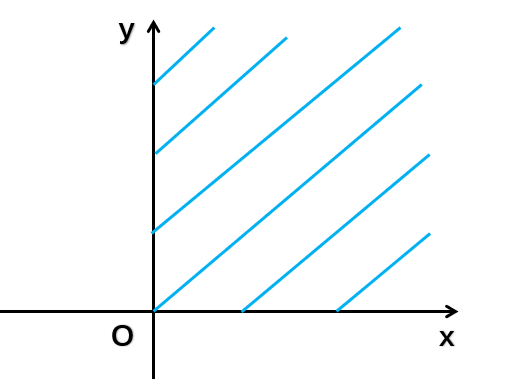
\includegraphics[scale=0.5]{figures/S5-1.png}
\end{center}
in this figure, it's NOT a vector space, because it's not closed, for example, under multiplication by real numbers
\vspace{14pt}
\newline
{\textcolor{anhao-scarlet}{a vector space has to be closed under}} multiplication and addition of vectors, in other words, {\textcolor{anhao-scarlet}{linear combination}}
\vspace{14pt}
\newline
$\mathbb{R}^n$ is the most important, but we will be interested in vector spaces that are inside $\mathbb{R}^n$, vector spaces that follow the rules
\begin{center}
	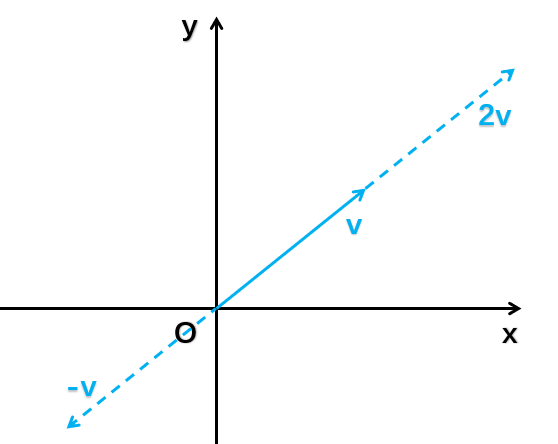
\includegraphics[scale=0.5]{figures/S5-2.png}
\end{center}
this is a vector space inside $\mathbb{R}^2$ (sub-space of $\mathbb{R}^2$)
\vspace{14pt}
\newline
what are the possible sub-spaces of $\mathbb{R}^2$?
\begin{enumerate}
	\item the whole space, $\mathbb{R}^2$ itself
	\item lines through 
		$\begin{bmatrix}
			0 \\
			0
		\end{bmatrix}$
	 (not the same as $\mathbb{R}^1$)
	\item zero vector only
\end{enumerate}
what are the possible sub-spaces of $\mathbb{R}^3$?
\begin{enumerate}
	\item $\mathbb{R}^3$
	\item plane through the origin
	\item line through the origin
	\item zero vector only
\end{enumerate}
\vspace{14pt}
how do sub-spaces come from matrices?
\vspace{14pt}
\newline
I want to create some sub-spaces out of this matrix: 
\begin{math}
	{\mathbf{A}} = 
	\begin{bmatrix}
		1 & 3 \\
		2 & 3 \\
		4 & 1
	\end{bmatrix}
\end{math}
\newline
all linear combinations of its columns (from $\mathbb{R}^3$) form a sub-space, called "column space", $C(\mathbf{A})$
\vspace{14pt}
\newline
the key idea is, we have to be able to take their combinations, still in the sub-space
\vspace{14pt}
\newline
if $col_1 // col_2$, then the column space is only a line through the origin

\newpage
\section{Lecture 06 - 列空间和零空间}
\pagestyle{fancy}
\lhead{}
\chead{Lecture 06 - 列空间和零空间}
\rhead{}

vector space requirements
\newline
$\Longleftrightarrow$ ${\mathbf{v+w}}$ and $c{\mathbf{v}}$ are in the space
\newline
$\Longleftrightarrow$ all combinations $c{\mathbf{v}}+d{\mathbf{w}}$ are in the space
\vspace{14pt}
\newline
notice that these two requirements mean
\newline
the sum and the scale of multiplication combine into linear combinations
\vspace{14pt}
\newline
Example: $\mathbb{R}^3$
\par 2 subspaces: $P$ - a plane, $L$ - a line
\par \ding{202} the union of those, $P \cup L$, has all vectors in $P$ or $L$ or both, is that a subspace?
\par NO!
\par \ding{203} the intersection, $P \cap L$, has all vectors that are in both, is that a subspace?
\par YES!
\par the general question is, I have subspaces $S$ and $T$, is their intersection $S \cap T$ a subspace?
\par YES!
\par proof:
\par\qquad if ${\mathbf{v}} \in S \cap T$, ${\mathbf{w}} \in S \cap T$
\par\qquad then ${\mathbf{v}}+{\mathbf{w}} \in S$ and ${\mathbf{v}}+{\mathbf{w}} \in T$
\par\qquad so ${\mathbf{v}}+{\mathbf{w}} \in S \cap T$
\par\qquad if ${\mathbf{v}} \in S \cap T$
\par\qquad then $c{\mathbf{v}} \in S$ and $c{\mathbf{v}} \in T$
\par\qquad so $c{\mathbf{v}} \in S \cap T$
\par in other words, when you take the intersection of two subspaces, 
\par you get probably a smaller subspace, but it is still a subspace
\vspace{31pt}
\newline
\begin{math}
	{\mathbf{A}} = 
	\begin{bmatrix}
		1 & 1 & 2 \\
		2 & 1 & 3 \\
		3 & 1 & 4 \\
		4 & 1 & 5
	\end{bmatrix}
\end{math}
\newline
the column space of ${\mathbf{A}}$, $C(\mathbf{A})$, is a subspace of $\mathbb{R}^4$
\newline
what's in that subspace?
\newline
not only the columns of ${\mathbf{A}}$, but also their linear combinations
\vspace{14pt}
\newline
so $C(\mathbf{A})$ is all linear combinations of ${\mathbf{A}}$'s columns
\vspace{14pt}
\newline
so I would like to know
\begin{math}
	\left\{
		\begin{array}{l}
			\text{what's in that space?} \\
			\text{how big is that space?} \\
			\text{is that the whole of 4-dim space? or is it a subspace inside?}
		\end{array}
	\right.
\end{math}
\newline
取三个四维向量进行线性组合,怎么也得不到整个四维空间嘛!
\vspace{14pt}
\newline
let's make this question connected with linear equations, 
\newline
does ${\mathbf{A}}{\mathbf{x}} = {\mathbf{b}}$ always have a solution for every ${\mathbf{b}}$?
\newline
NO, ${\mathbf{A}}{\mathbf{x}} = {\mathbf{b}}$ does not have a solution for every ${\mathbf{b}}$!
\vspace{14pt}
\newline
for example, 4 equations and 3 unknowns, 
\newline
(the combinations of 3 columns cannot always fill the 4-dim space)
\newline
there's going to be some ${\mathbf{b}}$, are not linear combinations of the 3 columns, but sometimes can
\vspace{14pt}
\newline
what ${\mathbf{b}}$'s allow me to solve ${\mathbf{A}}{\mathbf{x}} = {\mathbf{b}}$?
\vspace{14pt}
\newline
I can solve ${\mathbf{A}}{\mathbf{x}} = {\mathbf{b}}$ {\textcolor{anhao-scarlet}{exactly when 当且仅当}} the right-hand side ${\mathbf{b}}$ is a vector in $C(\mathbf{A})$. ( {\textcolor{anhao-scarlet}{OR}} ${\mathbf{b}}$ is a linear combination of ${\mathbf{A}}$'s columns. )
\vspace{14pt}
\newline
so, $C(\mathbf{A})$ consists of all vectors ${\mathbf{A}}{\mathbf{x}}$ ($\forall{\mathbf{x}}$)
\vspace{14pt}
\newline
if ${\mathbf{b}}$ is not a combination of ${\mathbf{A}}$'s columns, then there is no "${\mathbf{x}}$", there is no way to solve ${\mathbf{A}}{\mathbf{x}} = {\mathbf{b}}$
\vspace{14pt}
\newline
Example: 
\begin{math}
	{\mathbf{A}} = 
	\begin{bmatrix}
		1 & 1 & 2 \\
		2 & 1 & 3 \\
		3 & 1 & 4 \\
		4 & 1 & 5
	\end{bmatrix}
\end{math}
\par 
Question: Are those columns independent?
\vspace{14pt}
\par 
if I take the linear combinations of ${\mathbf{A}}$'s columns, does each column contributes something new or not? do I get a 3-D subspace?
\par 
NO!
\vspace{14pt}
\par 
can I throw away any column, and will get the same column space?
\par 
YES!
\vspace{14pt}
\par 
so for this ${\mathbf{A}}$, $C(\mathbf{A})$ is a 2-D subspace of $\mathbb{R}^4$
\vspace{31pt}
\newline
the null space 零空间 , is going to be a totally different subspace
\vspace{14pt}
\newline
the null space of ${\mathbf{A}}$, what's in it?
\begin{itemize}
	\item it contains not right-hand side ${\mathbf{b}}$
	\item it contains ${\mathbf{x}}$'s
	\item it contains all ${\mathbf{x}}$'s that solve "${\mathbf{A}}{\mathbf{x}} = {\mathbf{0}}$"
\end{itemize}
\vspace{14pt}
\begin{math}
	\begin{bmatrix}
		1 & 1 & 2 \\
		2 & 1 & 3 \\
		3 & 1 & 4 \\
		4 & 1 & 5 
	\end{bmatrix}
	\begin{bmatrix}
		x_1 \\
		x_2 \\
		x_3 
	\end{bmatrix}
	 = 
	\begin{bmatrix}
		0 \\
		0 \\
		0 \\
		0
	\end{bmatrix}
\end{math}
\newline
the null space certainly contains zero ($\because$ the null space is a vector space as well)
\newline
for this ${\mathbf{A}}$, 
\par\qquad $N({\mathbf{A}})$ contains 
\begin{math}
	\begin{bmatrix}
		0 \\
		0 \\
		0
	\end{bmatrix}
\end{math}
, 
\begin{math}
	\begin{bmatrix}
		1 \\
		1 \\
		-1
	\end{bmatrix}
\end{math}
, 
\begin{math}
	\begin{bmatrix}
		-4 \\
		-4 \\
		4
	\end{bmatrix}
\end{math}
, 
$\cdots$
, 
\begin{math}
	\begin{bmatrix}
		c \\
		c \\
		-c
	\end{bmatrix}
\end{math}
\par\qquad $N({\mathbf{A}})$ = 
\begin{math}
	c
	\begin{bmatrix}
		1 \\
		1 \\
		-1
	\end{bmatrix}
\end{math}
\par\qquad the null space is a line in $\mathbb{R}^3$
\vspace{14pt}
\par\qquad to check that the solutions to ${\mathbf{A}}{\mathbf{x}} = {\mathbf{0}}$ always give a subspace
\par\qquad proof:
\par\qquad\qquad if ${\mathbf{A}}{\mathbf{x}} = {\mathbf{0}}$ and ${\mathbf{A}}{\mathbf{x^*}} = {\mathbf{0}}$
\par\qquad\qquad then ${\mathbf{A}}({\mathbf{x}}+{\mathbf{x^*}}) = {\mathbf{0}}$
\par\qquad\qquad what's more, ${\mathbf{A}}(c{\mathbf{x}}) = c({\mathbf{A}}{\mathbf{x}})$
\vspace{31pt}
\newline
\begin{math}
	\begin{bmatrix}
		1 & 1 & 2 \\
		2 & 1 & 3 \\
		3 & 1 & 4 \\
		4 & 1 & 5 
	\end{bmatrix}
	\begin{bmatrix}
		x_1 \\
		x_2 \\
		x_3 
	\end{bmatrix}
	= 
	\begin{bmatrix}
		1 \\
		2 \\
		3 \\
		4
	\end{bmatrix}
\end{math}
\newline
I would like to know all the solutions to this equation, and if these solutions form a subspace?
\newline
NO! As zero vector is not a solution, and subspaces have to go through the origin.
\vspace{14pt}
\newline
{\textcolor{anhao-purple}{the solutions is a plane/line that does not go through the origin}}

\newpage
\section{Lecture 07 - 求解 Ax=0 :主变量与特解}
\pagestyle{fancy}
\lhead{}
\chead{Lecture 07 - 求解 Ax=0 :主变量与特解}
\rhead{}

\noindent what's the algorithm for solving ${\mathbf{A}}{\mathbf{x}} = {\mathbf{0}}$ ?
\vspace{14pt}
\newline
that's the null space that I'm interested in
\vspace{14pt}
\newline
\begin{math}
	{\mathbf{A}} = 
	\begin{bmatrix}
		1 & 2 & 2 & 2 \\
		2 & 4 & 6 & 8 \\
		3 & 6 & 8 & 10
	\end{bmatrix}
	\longrightarrow
	\begin{bmatrix}
		1 & 2 & 2 & 2 \\
		0 & 0 & 2 & 4 \\
		0 & 0 & 2 & 4 
	\end{bmatrix}
	\longrightarrow
	\begin{bmatrix}
		1 & 2 & 2 & 2 \\
		0 & 0 & 2 & 4 \\
		0 & 0 & 0 & 0 
	\end{bmatrix}
	 = 
	{\mathbf{U}}
\end{math}
\newline
while I am doing elimination, 
\newline
I am not changing the solutions $\Longrightarrow$ I am not changing the null space
\vspace{14pt}
\newline
\begin{math}
	\begin{bmatrix}
		 & 1 &   & 2 &   & 2 &   & 2 & \\
		 & {\textcolor{anhao-sky}{=}} & {\textcolor{anhao-sky}{=}} & {\textcolor{anhao-sky}{=}} & {\textcolor{anhao-sky}{=}} &   &   &   & \\
		 & 0 &   & 0 & {\textcolor{anhao-sky}{||}} & 2 &   & 4 & \\
		 &   &   &   & {\textcolor{anhao-sky}{=}} & {\textcolor{anhao-sky}{=}} & {\textcolor{anhao-sky}{=}} & {\textcolor{anhao-sky}{=}} & \\
		 & 0 &   & 0 &   & 0 &   & 0 & 
	\end{bmatrix}
\end{math}
 : echelon form, staircase form
\newline
there are two pivots only
\vspace{14pt}
\newline
{\textcolor{anhao-scarlet}{the number of pivots = the rank of the matrix = the number of pivot variables}}
\vspace{14pt}
\newline
\begin{math}
	{\mathbf{A}}{\mathbf{x}} = {\mathbf{0}}
	\Longrightarrow
	{\mathbf{U}}{\mathbf{x}} = {\mathbf{0}}
\end{math}
\qquad {\textcolor{anhao-scarlet}{same solutions, same null space}}
\vspace{14pt}
\newline
how do I describe the solutions?
\newline
四个三维向量一定线性相关
\vspace{14pt}
\newline
\begin{math}
	\begin{bmatrix}
		{\textcolor{blue}{\boxed{1}}} & {\textcolor{anhao-orange}{2}} & {\textcolor{blue}{2}} & {\textcolor{anhao-orange}{2}} \\
		{\textcolor{blue}{0}} & {\textcolor{anhao-orange}{0}} & {\textcolor{blue}{\boxed{2}}} & {\textcolor{anhao-orange}{4}} \\
		{\textcolor{blue}{0}} & {\textcolor{anhao-orange}{0}} & {\textcolor{blue}{0}} & {\textcolor{anhao-orange}{0}} 
	\end{bmatrix}
\end{math}
\qquad
2 {\textcolor{anhao-orange}{free columns}}, 
2 {\textcolor{blue}{pivot columns}}
\newline
{\bf{free}} means that we can assign values freely, and we can find the other values accordingly
\vspace{14pt}
\newline
for convenient purpose, we choose 1 and 0 to those free variables
\vspace{14pt}
\newline
\begin{math}
	{\mathbf{x_1}} = 
	\begin{bmatrix}
		-2 \\
		{\textcolor{anhao-scarlet}{1}} \\
		0 \\
		{\textcolor{anhao-scarlet}{0}}
	\end{bmatrix}
\end{math}
 , 
\begin{math}
	{\mathbf{x_2}} = 
	\begin{bmatrix}
		2 \\
		{\textcolor{anhao-scarlet}{0}} \\
		-2 \\
		{\textcolor{anhao-scarlet}{1}}
	\end{bmatrix}
\end{math}
\qquad
2 special solutions (I gave special numbers to free variables)
\newline
what are all the solutions to ${\mathbf{A}}{\mathbf{x}} = {\mathbf{0}}$ or ${\mathbf{U}}{\mathbf{x}} = {\mathbf{0}}$ ?
\newline
\begin{math}
	{\mathbf{x}} = 
	c
	\begin{bmatrix}
		-2 \\
		{\textcolor{anhao-scarlet}{1}} \\
		0 \\
		{\textcolor{anhao-scarlet}{0}}
	\end{bmatrix}
	 + 
	d
	\begin{bmatrix}
		2 \\
		{\textcolor{anhao-scarlet}{0}} \\
		-2 \\
		{\textcolor{anhao-scarlet}{1}}
	\end{bmatrix}
	 = 
	c{\mathbf{x_1}} + d{\mathbf{x_2}}
\end{math}
\newline
I am taking all the linear combinations of my 2 special solutions, and they are null space.
\vspace{14pt}
\newline
how many special solution are there? 每个自由变量对应一个特解
\vspace{14pt}
\newline
\begin{math}
	\begin{bmatrix}
		\ & \ & \ & \ & \ \\
		\ & \ & \ & \ & \ 
	\end{bmatrix}_{m \times n}
\end{math}
 with rank $r$, $(n-r)$ free variables
\newline
we get $r$ pivot variables, so there are really $r$ equations there, only $r$ independent equations, and there are $(n-r)$ variables that we can choose freely
\vspace{14pt}
\newline
Algorithms to Solve ${\mathbf{A}}{\mathbf{x}} = {\mathbf{0}}$
\begin{enumerate}
	\item do elimination
	\item decide which are pivot columns and which are free columns
	\item give values to free variables
	\item complete pivot values accordingly
	\item do linear combinations
\end{enumerate}
\vspace{14pt}
reduced row echelon form (${\mathbf{U}}$ 还可以简化)
\newline
\begin{math}
	{\mathbf{U}} = 
	\begin{bmatrix}
		1 & 2 & 2 & 2 \\
		0 & 0 & 2 & 4 \\
		0 & 0 & 0 & 0 
	\end{bmatrix}
	\longrightarrow
	\begin{bmatrix}
		1 & 2 & 0 & -2 \\
		0 & 0 & 2 & 4 \\
		0 & 0 & 0 & 0 
	\end{bmatrix}
	\longrightarrow
	\begin{bmatrix}
		{\boxed{1}} & 2 & 0 & -2 \\
		0 & 0 & {\boxed{1}} & 2 \\
		0 & 0 & 0 & 0 
	\end{bmatrix}
	 = 
	{\mathbf{R}}
\end{math}
\newline
in rref, it has zeros above and below the pivots
\vspace{14pt}
\newline
\begin{math}
	\begin{bmatrix}
		{\boxed{1}} & 2 & 0 & -2 \\
		0 & 0 & {\boxed{1}} & 2 \\
		0 & 0 & 0 & 0 
	\end{bmatrix}
\end{math}
\newline
notice that there is an identity sitting in the pivot rows and pivot columns!
\vspace{14pt}
\newline
\begin{math}
	{\mathbf{A}}{\mathbf{x}} = {\mathbf{0}}
	\Longrightarrow
	{\mathbf{U}}{\mathbf{x}} = {\mathbf{0}}
	\Longrightarrow
	{\mathbf{R}}{\mathbf{x}} = {\mathbf{0}}
\end{math}
\vspace{31pt}
\newline
\begin{math}
	{\mathbf{A}} = 
	\begin{bmatrix}
		1 & 2 & 2 & 2 \\
		2 & 4 & 6 & 8 \\
		3 & 6 & 8 & 10
	\end{bmatrix}
\end{math}
\newline
\begin{math}
	{\mathbf{A^{T}}} = 
	\begin{bmatrix}
		1 & 2 & 3 \\
		2 & 4 & 6 \\
		2 & 6 & 8 \\
		2 & 8 & 10
	\end{bmatrix}
	\longrightarrow
	\begin{bmatrix}
		1 & 2 & 3 \\
		0 & 0 & 0 \\
		0 & 2 & 2 \\
		0 & 4 & 4
	\end{bmatrix}
	\longrightarrow
	\begin{bmatrix}
		1 & 2 & 3 \\
		0 & 1 & 1 \\
		0 & 0 & 0 \\
		0 & 0 & 0
	\end{bmatrix}
	\longrightarrow
	\begin{bmatrix}
		1 & 0 & 1 \\
		0 & 1 & 1 \\
		0 & 0 & 0 \\
		0 & 0 & 0
	\end{bmatrix}
\end{math}
\newline
so the rank is 2 again!
\newline
the number of special solutions is 1
\vspace{14pt}
\newline
{\textcolor{anhao-scarlet}{the fact: the number of pivot columns of ${\mathbf{A}}$ and ${\mathbf{A^{T}}}$ is the same}}

\newpage
\section{Lecture 08 - 可解性与解的结构}
\pagestyle{fancy}
\lhead{}
\chead{Lecture 08 - 可解性与解的结构}
\rhead{}

\noindent
\begin{math}
	\left\{  
	\begin{array}{rclrclrclrcl}
		1x_1 & + & 2x_2 & + & 2x_3 & + & 2x_4 & = & b_1 \\
		2x_1 & + & 4x_2 & + & 6x_3 & + & 8x_4 & = & b_2 \\
		3x_1 & + & 6x_2 & + & 8x_3 & + & 10x_4 & = & b_3
	\end{array}  
	\right.
\end{math}
\newline
there is a condition on $b_1$, $b_2$, $b_3$ for this system to have a solution
\vspace{14pt}
\newline
\begin{math}
	\underbrace{
		\left[
			\begin{array}{cccc|c}
				1 & 2 & 2 & 2 & b_1 \\
				2 & 4 & 6 & 8 & b_2 \\
				3 & 6 & 8 & 10 & b_3 
			\end{array}
		\right]
	}_{
		{\text{augmented matrix}} = 
		\left[
			\begin{array}{c|c}
				{\mathbf{A}} & {\mathbf{b}}
			\end{array}
		\right]
	}
	\longrightarrow
	\left[
	\begin{array}{cccc|l}
		1 & 2 & 2 & 2 & b_1 \\
		0 & 0 & 2 & 4 & b_2-2b_1 \\
		0 & 0 & 2 & 4 & b_3-3b_1 
	\end{array}
	\right]
	\longrightarrow
	\left[
	\begin{array}{cccc|l}
		1 & 2 & 2 & 2 & b_1 \\
		0 & 0 & 2 & 4 & b_2-2b_1 \\
		0 & 0 & 0 & 0 & b_3-b_2-b_1 
	\end{array}
	\right]
\end{math}
\newline
$b_3-b_2-b_1=0$, this is the condition for solvability
\newline
suppose that 
\begin{math}
	{\mathbf{b}} = 
	\begin{bmatrix}
		1 \\
		5 \\
		6 
	\end{bmatrix}
\end{math}
 , 
\newline
\begin{math}
	\left[
	\begin{array}{c|c}
		{\mathbf{A}} & {\mathbf{b}}
	\end{array}
	\right]
	\longrightarrow
	\left[
	\begin{array}{cccc|c}
		1 & 2 & 2 & 2 & 1 \\
		0 & 0 & 2 & 4 & 3 \\
		0 & 0 & 0 & 0 & 0 
	\end{array}
	\right]
\end{math}
\vspace{14pt}
\newline
what are the conditions on ${\mathbf{b}}$ that make the equation system solvable?
\vspace{14pt}
\newline
Solvability Condition on ${\mathbf{b}}$
\begin{itemize}
	\item 表述一
	\par 当且仅当 ${\mathbf{b}}$ 属于 ${\mathbf{A}}$ 的列空间时成立 
	\par 或者 ${\mathbf{b}}$ 必须是 ${\mathbf{A}}$ 各列的线性组合
	\item 表述二
	\par if a combination of the rows of ${\mathbf{A}}$ gives the zero row,
	\par the same combination of the components of ${\mathbf{b}}$ has to give zero
\end{itemize}
\vspace{14pt}
what's the algorithm to find the solutions?
\begin{enumerate}
	\item a particular solution, ${\mathbf{x}}_{particular}$
	\par to set all free variables to zero, 
	\par since those free variables can be anything,
	\par then solve ${\mathbf{A}}{\mathbf{x}} = {\mathbf{b}}$ to get the pivot variables
	\par in this case, 
	\begin{math}
		{\mathbf{x}}_p = 
		\begin{bmatrix}
			-2 \\
			0 \\
			3/2 \\
			0 
		\end{bmatrix}
	\end{math}
	\item ${\mathbf{x}}$ from null space, ${\mathbf{x}}_{nullspace}$
	\par in this case, 
	\begin{math}
		{\mathbf{x}}_n = 
		c_1
		\begin{bmatrix}
			-2 \\
			1 \\
			0 \\
			0 
		\end{bmatrix}
		 + 
		c_2
		\begin{bmatrix}
			2 \\
			0 \\
			-2 \\
			1 
		\end{bmatrix}
	\end{math}
	\item ${\mathbf{x}}_{c}={\mathbf{x}}_{p}+{\mathbf{x}}_{n}$, ${\mathbf{x}}_{complete}$
	\par in this case, 
	\begin{math}
		{\mathbf{x}}_c = 
		\begin{bmatrix}
			-2 \\
			0 \\
			3/2 \\
			0 
		\end{bmatrix}
		 + 
		c_1
		\begin{bmatrix}
			-2 \\
			1 \\
			0 \\
			0 
		\end{bmatrix}
		+ 
		c_2
		\begin{bmatrix}
			2 \\
			0 \\
			-2 \\
			1 
		\end{bmatrix}
	\end{math}
\end{enumerate}
\begin{center}
	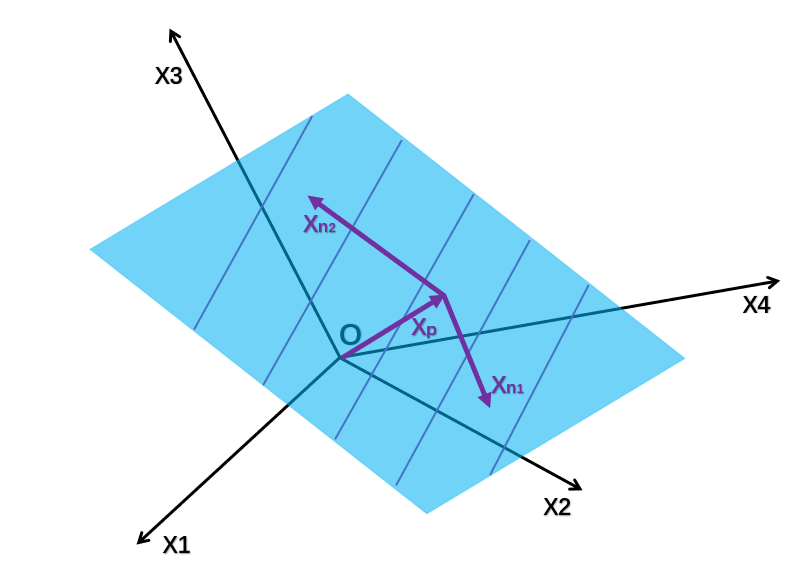
\includegraphics[scale=0.8]{figures/S8-1.png}
	\newline
	{\textcolor{anhao-scarlet}{“由零空间这个子空间从原点平移过来得到的平面”}}
\end{center}
\vspace{31pt}
think of a $m \times n$ matrix ${\mathbf{A}}$ of rank $r$, 
\begin{math}
	\left\{
		\begin{array}{rcl}
			r \leq m \\
			r \leq n 
		\end{array}
	\right.
\end{math}
\newline
\begin{itemize}
	\item full column rank ( $r=n$ )
	\par 意味着全部向量撑开全部的维数
	\par there's a pivot in every column, no free variables
	\par there are no free variables to give values, so the null space is only the zero vector
	\par i.e. $N({\mathbf{A}})=\left\{{\mathbf{0}}\right\}$
	\par the complete solution to ${\mathbf{A}}{\mathbf{x}} = {\mathbf{b}}$ is just ${\mathbf{x}}_p$, it's the unique solution if ${\mathbf{x}}_p$ exists
	\par “列满秩时,如果解存在(${\mathbf{b}} \in C({\mathbf{A}})$),那么解唯一” “此时只有零个解或一个解”
	\item full row rank ( $r=m$ )
	\par every row has a pivot
	\par I can solve ${\mathbf{A}}{\mathbf{x}} = {\mathbf{b}}$ for any ${\mathbf{b}}$
	\par “在消元时没有得到零行!”
	\par number(free-variables) = $n-m$
	\item $r=m=n$ 
	\par invertible!
	\par 此时 ${\mathbf{A}}{\mathbf{x}} = {\mathbf{b}}$ 必定有解且解唯一
	\item $r<m$ and $r<n$
	\par 0 solution or $\infty$ solutions
\end{itemize}

\newpage
\section{Lecture 09 - 线性相关性、基、维数}
\pagestyle{fancy}
\lhead{}
\chead{Lecture 09 - 线性相关性、基、维数}
\rhead{}

\noindent key words:
\begin{itemize}
	\item linear independence
	\item spanning a space
	\item basis for a subspace / basis for a vector space
	\item the dimension of a subspace
\end{itemize}
we talk about a bunch of vectors 
\begin{math}
	\left\{
		\begin{array}{l}
			{\text{being independent}} \\
			{\text{spanning a space}} \\
			{\text{being a basis}}
		\end{array}
	\right.
\end{math}
\vspace{14pt}
\newline
suppose ${\mathbf{A}}$ is a $m \times n$ ($m < n$) matrix, ($\#unknowns > \#equations$)
\newline
then there are non-zero solutions to ${\mathbf{A}}{\mathbf{x}} = {\mathbf{0}}$
\newline
$\Longrightarrow$ 在 ${\mathbf{A}}$ 的零空间中,除了零向量之外,还包含了其他一些向量
\vspace{14pt}
\newline
the reason is, there will be free variables, at least one, which I can assign non-zero values to
\vspace{14pt}
\newline
vectors ${\mathbf{x_1}}$, ${\mathbf{x_2}}$, $\cdots$ , ${\mathbf{x_n}}$ are independent if no combination, except the "zero combination", gives the zero vector
\begin{center}
	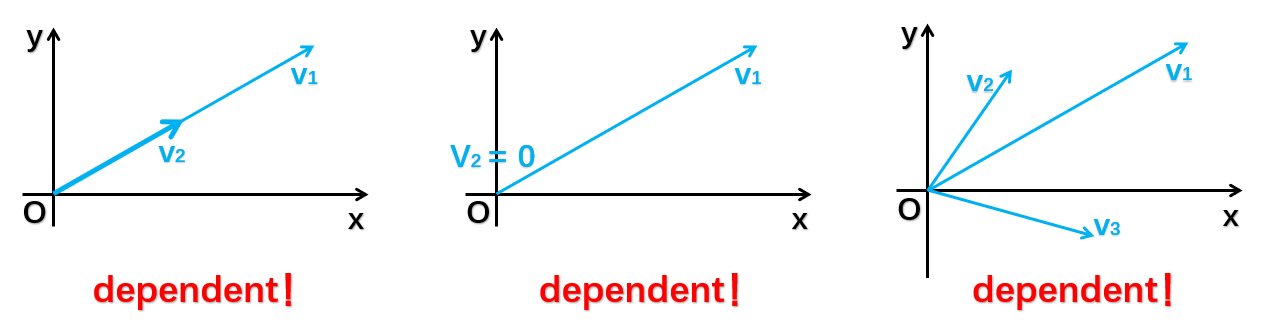
\includegraphics[scale=0.6]{figures/S9-1.png}
\end{center}
{\textcolor{anhao-purple}{\bf{corollary}}}
\begin{itemize}
	\item if the zero vector is in there, "independent is dead"
	\item 如果零空间 $N({\mathbf{A}})$ 里存在非零向量,那么各列相关
\end{itemize}
\vspace{14pt}
when ${\mathbf{v_1}}$, ${\mathbf{v_2}}$, $\cdots$ , ${\mathbf{v_n}}$ are columns of ${\mathbf{A}}$,
\newline
they are independent if null space of ${\mathbf{A}}$ is only the zero vector, $rank=n$, NO free variables,
\newline
they are dependent if there exists non-zero ${\mathbf{c}}$, such that ${\mathbf{A}}{\mathbf{c}}={\mathbf{0}}$, $rank<n$, YES free variables
\vspace{14pt}
\newline
vectors ${\mathbf{v_1}}$, ${\mathbf{v_2}}$, $\cdots$ , ${\mathbf{v_l}}$ span a space means,
\newline
the space consists of all combinations of those vectors,
\newline
the space will be the smallest space with those combinations in it
\vspace{14pt}
\newline
the column space of a matrix, is the space spanned by its columns
\vspace{14pt}
\newline
a basis for a vector space is a sequence of vectors, ${\mathbf{v_1}}$, ${\mathbf{v_2}}$, $\cdots$ , ${\mathbf{v_d}}$, with 2 properties:
\newline
{\textcolor{anhao-scarlet}{(向量的个数刚刚好)}}
\begin{itemize}
	\item they are independent
	\item they can span the space
\end{itemize}
\vspace{14pt}
Example: space is $\mathbb{R}^3$
\par one basis is 
\begin{math}
	\begin{bmatrix}
		1 \\
		0 \\
		0 
	\end{bmatrix}
\end{math}
, 
\begin{math}
	\begin{bmatrix}
		0 \\
		1 \\
		0 
	\end{bmatrix}
\end{math}
, 
\begin{math}
	\begin{bmatrix}
		0 \\
		0 \\
		1 
	\end{bmatrix}
\end{math}
\par another basis is 
\begin{math}
	\begin{bmatrix}
		1 \\
		1 \\
		2 
	\end{bmatrix}
\end{math}
, 
\begin{math}
	\begin{bmatrix}
		2 \\
		2 \\
		5 
	\end{bmatrix}
\end{math}
, 
\begin{math}
	\begin{bmatrix}
		3 \\
		4 \\
		5 
	\end{bmatrix}
\end{math}
\vspace{14pt}
\newline
{\textcolor{anhao-purple}{for $\mathbb{R}^n$, $n$ vectors give a basis if the $n \times n$ matrix with those columns is invertible}}
\vspace{14pt}
\newline
{\textcolor{anhao-purple}{the basis is not unique, for $\mathbb{R}^3$, any invertible $3 \times 3$ matrix, its columns are a basis for $\mathbb{R}^3$}}
\vspace{14pt}
\newline
but there is a common character of those bases, that's the number of vectors!
\vspace{14pt}
\newline
{\textcolor{anhao-purple}{Given a space, every basis for the space has the same number\footnote{Def. dimension of the space} of vectors.}}
\vspace{14pt}
\newline
Example: 
\begin{math}
	{\mathbf{A}} = 
	\begin{bmatrix}
		1 & 2 & 3 & 1 \\
		1 & 1 & 2 & 1 \\
		1 & 2 & 3 & 1 
	\end{bmatrix}
\end{math}
\par one of the bases for $C({\mathbf{A}})$ is 
\begin{math}
	\left\{
	\begin{bmatrix}
		1 \\
		1 \\
		1 
	\end{bmatrix}
	, 
	\begin{bmatrix}
		2 \\
		1 \\
		2 
	\end{bmatrix}
	\right\}
\end{math}
\par one of the bases for $N({\mathbf{A}})$ is 
\begin{math}
	\left\{
	\begin{bmatrix}
		-1 \\
		-1 \\
		1 \\
		0 
	\end{bmatrix}
	, 
	\begin{bmatrix}
		-1 \\
		0 \\
		0 \\
		1 
	\end{bmatrix}
	\right\}
\end{math}
\par the rank of ${\mathbf{A}}$ is $2$ = the number of pivot columns = the dimension of $C({\mathbf{A}})$
\vspace{14pt}
\newline
{\textcolor{anhao-scarlet}{$dim \ C({\mathbf{A}}) = rank({\mathbf{A}}) = r$}}
\newline
{\textcolor{anhao-scarlet}{$dim \ N({\mathbf{A}}) = the \ number \ of \ free \ variables = n - r$}}
\vspace{14pt}
\newline
{\textcolor{anhao-scarlet}{行秩等于列秩!}}
\vspace{14pt}
\newline
standard basis for $\mathbb{R}^3$ is 
\begin{math}
	\left\{
	\begin{bmatrix}
		1 \\
		0 \\
		0 
	\end{bmatrix}
	, 
	\begin{bmatrix}
		0 \\
		1 \\
		0 
	\end{bmatrix}
	, 
	\begin{bmatrix}
		0 \\
		0 \\
		1 
	\end{bmatrix}
	\right\}
\end{math}

\newpage
\section{Lecture 10 - 四个基本子空间}
\pagestyle{fancy}
\lhead{}
\chead{Lecture 10 - 四个基本子空间}
\rhead{}

\noindent 4 fundamental subspaces of ${\mathbf{A}}_{m \times n}$
\begin{itemize}
	\item the column space, $C({\mathbf{A}})$, $C({\mathbf{A}}) \subset \mathbb{R}^m$
	\item the null space, $N({\mathbf{A}})$, $N({\mathbf{A}}) \subset \mathbb{R}^n$
	\item the row space, it's all the combinations of the rows, $C({\mathbf{A^{T}}})$, $C({\mathbf{A^{T}}}) \subset \mathbb{R}^n$
	\item the null space of ${\mathbf{A^{T}}}$, $N({\mathbf{A^{T}}})$, the left null space of ${\mathbf{A}}$, $N({\mathbf{A^{T}}}) \subset \mathbb{R}^m$
\end{itemize}
\begin{center}
	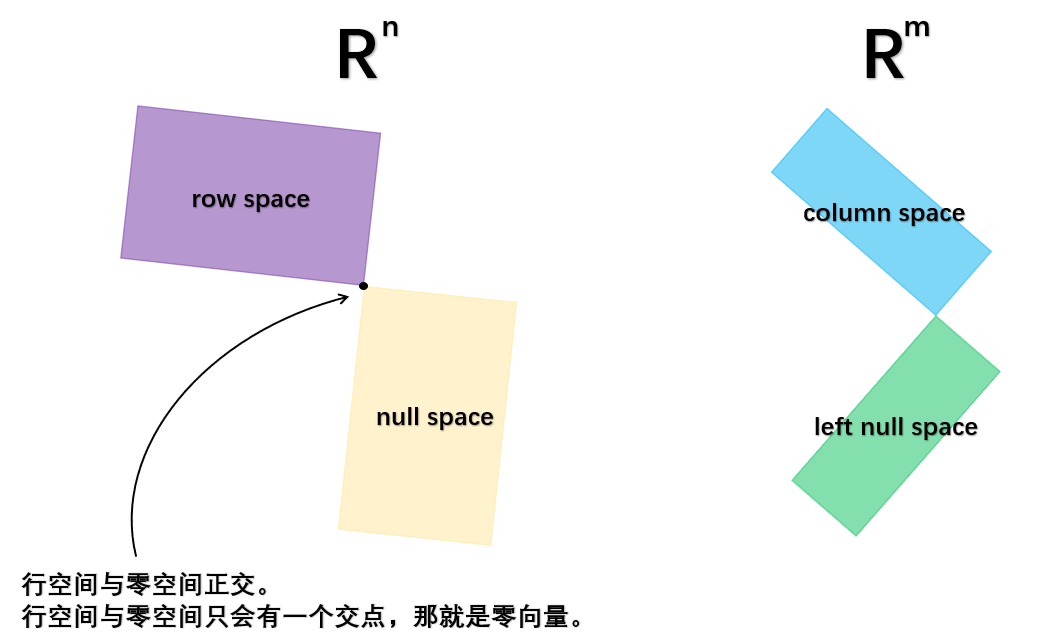
\includegraphics[scale=0.8]{figures/S10-1.png}
\end{center}
\begin{center}
	\begin{tabular}{ c c c c c }
		\toprule
		\ & $C({\mathbf{A}})$ & $C({\mathbf{A^{T}}})$ & $N({\mathbf{A}})$ & $N({\mathbf{A^{T}}})$ \\
		\toprule
		basis & the pivot columns & the first $r$ rows of ${\mathbf{R}}$ & the special solutions & \ \\
		\hline
		dimension & rank $r$ & rank $r$ & $n-r$ & $m-r$ \\
		\bottomrule
	\end{tabular}
\end{center}
{\textcolor{anhao-scarlet}{the row space and the column space have the same dimension!}}
\vspace{14pt}
\newline
\begin{math}
	{\mathbf{A}} \xrightarrow{\quad rref() \quad} {\mathbf{R}}
\end{math}
\quad different column space, same row space
\newline
{\textcolor{anhao-scarlet}{因为 ${\mathbf{R}}$ 是由 ${\mathbf{A}}$ 经过行变化而来,所以它们共享同一个行空间。}}

\newpage
\section{Lecture 14 - 正交向量与子空间}
\pagestyle{fancy}
\lhead{}
\chead{Lecture 14 - 正交向量与子空间}
\rhead{}

\noindent key words:
\begin{itemize}
	\item orthogonal vectors
	\item orthogonal subspaces
	\item orthogonal bases
\end{itemize}
\begin{center}
	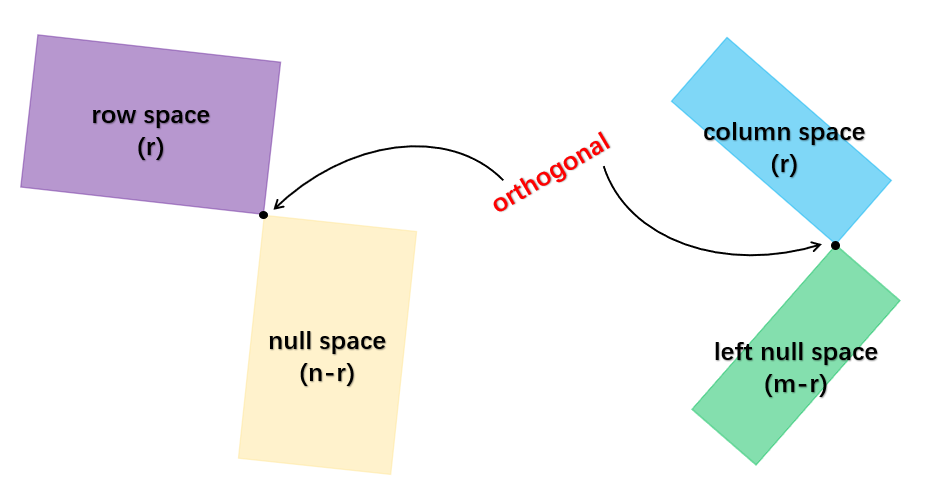
\includegraphics[scale=0.75]{figures/S14-1.png}
\end{center}
\vspace{14pt}
orthogonal(perpendicular) vectors: ${\mathbf{x^{T}}}{\mathbf{y}} = {\mathbf{0}}$
\newline
proof:
\par $\because \Vert{\mathbf{x}}\Vert^2 + \Vert{\mathbf{y}}\Vert^2 = \Vert{\mathbf{x+y}}\Vert^2$ \quad (Pythagoras)
\par 即 ${\mathbf{x^{T}}}{\mathbf{x}} + {\mathbf{y^{T}}}{\mathbf{y}} = {\mathbf{(x+y)^{T}}}{\mathbf{(x+y)}}$
\par $\Leftrightarrow {\mathbf{x^{T}}}{\mathbf{x}} + {\mathbf{y^{T}}}{\mathbf{y}} = {\mathbf{(x^T+y^T)}}{\mathbf{(x+y)}}$
\par $\therefore {\mathbf{x^{T}}}{\mathbf{y}} + {\mathbf{x}}{\mathbf{y^{T}}} = {\mathbf{0}}$
\par $\because {\mathbf{x^{T}}}{\mathbf{y}} = {\mathbf{x}}{\mathbf{y^{T}}}$
\par $\therefore {\mathbf{x^{T}}}{\mathbf{y}} = {\mathbf{0}}$
\par Q.E.D.
\vspace{14pt}
\newline
subspace $S$ is orthogonal to subspace $T$, 
\par means that every vector in $S$ is orthogonal to every vector in $T$
\begin{center}
	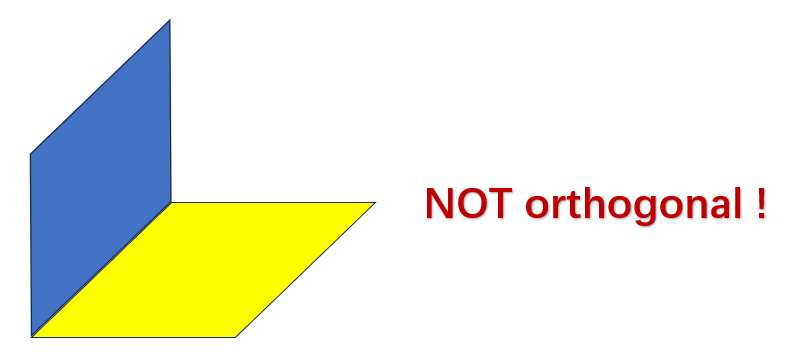
\includegraphics[scale=0.4]{figures/S14-2.png}
\end{center}
"non-zero vectors are not orthogonal to themselves"
\newline
"if two subspaces meet at some non-zero vectors, they are not orthogonal"
\vspace{14pt}
\newline
row space is orthogonal to null space, why?
\par ${\mathbf{A}}{\mathbf{x}}={\mathbf{0}}$
\par 
\begin{math}
	\begin{bmatrix}
		\quad & row_1 & \quad \\
		\quad & row_2 & \quad \\
		\quad & \cdots & \quad \\
		\quad & row_m & \quad \\
	\end{bmatrix}
	\begin{bmatrix}
		\quad & x_1 & \quad \\
		\quad & x_2 & \quad \\
		\ & \ & \ \\
		\quad & \vdots & \quad \\
		\ & \ & \ \\
		\quad & x_n & \quad \\
	\end{bmatrix}
	 = 
	\begin{bmatrix}
		\quad & 0 & \quad \\
		\quad & 0 & \quad \\
		\ & \ & \ \\
		\quad & \vdots & \quad \\
		\ & \ & \ \\
		\quad & 0 & \quad \\
	\end{bmatrix}
\end{math}
\par therefore,
\par\qquad $c_1{\mathbf{(row_1)^T}}{\mathbf{x}} = 0$
\par\qquad $c_2{\mathbf{(row_2)^T}}{\mathbf{x}} = 0$
\par\qquad $\cdots\quad\cdots\quad\cdots$
\par\qquad $c_m{\mathbf{(row_m)^T}}{\mathbf{x}} = 0$
\par $\therefore \left[ c_1{\mathbf{(row_1)^T}} + c_2{\mathbf{(row_2)^T}} + \cdots + c_m{\mathbf{(row_m)^T}} \right]{\mathbf{x}} = {\mathbf{0}}$
\par $\therefore \left[ c_1{\mathbf{row_1}} + c_2{\mathbf{row_2}} + \cdots + c_m{\mathbf{row_m}} \right]^{\mathbf{T}}{\mathbf{x}} = {\mathbf{0}}$
\par Q.E.D.
\vspace{14pt}
\newline
{\textcolor{anhao-scarlet}{正交子空间可以不同维!}}
\vspace{14pt}
\newline
null space and row space are orthogonal complements (补集) in $\mathbb{R}^n$
\newline
注:空间的正交补,包含了所有与之正交的向量,而不只是部分。
\newline
null space contains all, not just some, vectors that are perpendicular to row space

\newpage
\section{Lecture 15 - 子空间投影}
\pagestyle{fancy}
\lhead{}
\chead{Lecture 15 - 子空间投影}
\rhead{}

\noindent “如何求一个无解的方程组的解?” (回归问题、拟合、坏数据)
\newline
"solve" ${\mathbf{A}}{\mathbf{x}} = {\mathbf{b}}$ when there is no solution, what's the best solution?
\vspace{14pt}
\newline
{\textcolor{anhao-scarlet}{${\mathbf{A^{T}}}{\mathbf{A}}$ is symmetric}}
\newline
proof:
\par $({\mathbf{A^{T}}}{\mathbf{A}})^{\mathbf{T}} = {\mathbf{A^{T}}}{\mathbf{A^{TT}}} = {\mathbf{A^{T}}}{\mathbf{A}}$
\vspace{14pt}
\newline
{\textcolor{anhao-scarlet}{$rank({\mathbf{A^{T}}}{\mathbf{A}}) = rank({\mathbf{A}})$}}
\vspace{14pt}
\newline
{
	\textcolor{anhao-scarlet}
	{
		$rank({\mathbf{A}}{\mathbf{B}}) \leq min \{ rank({\mathbf{A}}), rank({\mathbf{B}}) \}$
	}
}
\vspace{14pt}
\newline
\begin{math}
	{\mathbf{A}}{\mathbf{x}} = {\mathbf{b}}
	\longrightarrow
	{\mathbf{A^{T}}}{\mathbf{A}}{\mathbf{\hat{x}}} = {\mathbf{A^{T}}}{\mathbf{b}}
\end{math}
\vspace{14pt}
\newline
{
	\textcolor{anhao-scarlet}
	{
		${\mathbf{A^{T}}}{\mathbf{A}}$ 不一定是可逆的
	}
}
,例如零矩阵,或者
\begin{math}
	\begin{bmatrix}
		1 & 3 \\
		1 & 3 \\
		1 & 3 
	\end{bmatrix}
\end{math}
\newline
{
	\textcolor{anhao-scarlet}
	{
		${\mathbf{A^{T}}}{\mathbf{A}}$ is invertible exactly if ${\mathbf{A}}$ has independent columns
	}
}
\vspace{31pt}
\newline
考虑二维的情况
\begin{center}
	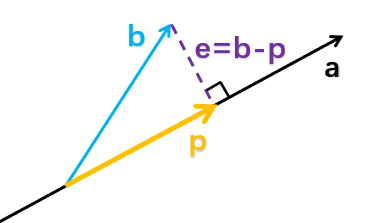
\includegraphics[scale=0.8]{figures/S15-1.png}
\end{center}
\begin{math}
	{\mathbf{a^{T}}}{\mathbf{e}} = {\mathbf{a^{T}}}({\mathbf{b}}-{\mathbf{p}}) = {\mathbf{a^{T}}}({\mathbf{b}}-\lambda{\mathbf{a}}) = 0
\end{math}
\newline
\begin{math}
	\Longrightarrow
	\lambda{\mathbf{a^{T}}}{\mathbf{a}} = {\mathbf{a^{T}}}{\mathbf{b}}
\end{math}
\newline
\begin{math}
	\Longrightarrow
	\lambda = \cfrac{{\mathbf{a^{T}}}{\mathbf{b}}}{{\mathbf{a^{T}}}{\mathbf{a}}}
	\in {\mathbb{R}}
\end{math}
\newline
\begin{math}
	\Longrightarrow
	{\mathbf{p}} = \lambda\cdot{\mathbf{a}} = {\mathbf{a}}\cdot\lambda = {\mathbf{a}}\cdot\cfrac{{\mathbf{a^{T}}}{\mathbf{b}}}{{\mathbf{a^{T}}}{\mathbf{a}}} = 
	\cfrac{{\mathbf{a}}{\mathbf{a^{T}}}}{{\mathbf{a^{T}}}{\mathbf{a}}}\cdot{\mathbf{b}} = {\mathbf{P}}{\mathbf{b}}
\end{math}
\vspace{14pt}
\newline
${\mathbf{P}}$ is the projection matrix acting on the input, ${\mathbf{P}}^2={\mathbf{P}}$, ${\mathbf{P^{T}}}={\mathbf{P}}$
\newline
if ${\mathbf{b}}$ is doubled, ${\mathbf{p}}$ will be doubled
\newline
if ${\mathbf{a}}$ is doubled, ${\mathbf{p}}$ will not change at all
\vspace{31pt}
\newline
为什么这里要引入投影矩阵?
\newline
$\because$ ${\mathbf{A}}{\mathbf{x}}={\mathbf{b}}$ may have no solutions
\newline
$\therefore$ I turn to solve the closest problem that I can solve
\newline
$\because$ ${\mathbf{A}}{\mathbf{x}}$ will always be in the column space of ${\mathbf{A}}$, but ${\mathbf{b}}$ is probably not
\newline
(所以我要怎么微调 ${\mathbf{b}}$ ?)
\newline
$\therefore$ solve ${\mathbf{A}}{\mathbf{\hat{x}}}={\mathbf{p}}$ instead, where ${\mathbf{p}}$ is the projection of ${\mathbf{b}}$ onto the column space
\vspace{31pt}
\newline
考虑三维的情况
\begin{center}
	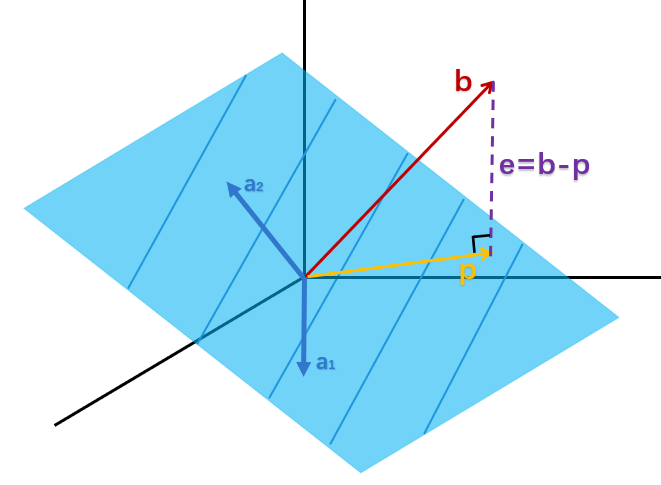
\includegraphics[scale=0.8]{figures/S15-2.png}
\end{center}
$\left\{{\mathbf{a_1}}, {\mathbf{a_2}}\right\}$ is a basis for the plane, plane is the column space of ${\mathbf{A}}$
\newline
若 ${\mathbf{b}}$ 不在列空间中,则投影到列空间里,若 ${\mathbf{b}}$ 在列空间中,则投影结果就是 ${\mathbf{b}}$ 自己
\newline
${\mathbf{e}}$ is perpendicular to the plane
\newline
投影 ${\mathbf{p}}$ 是基向量 $\left\{{\mathbf{a_1}}, {\mathbf{a_2}}\right\}$ 的线性组合,${\mathbf{p}} = \hat{x_1}{\mathbf{a_1}} + \hat{x_2}{\mathbf{a_2}}$(在${\mathbf{a_1}}$方向和${\mathbf{a_2}}$方向的投影之和)
\vspace{31pt}
\newline
如前文所说,我们改为求解 ${\mathbf{A}}{\mathbf{\hat{x}}}={\mathbf{p}}$ (to find ${\mathbf{\hat{x}}}$)
\newline
key: ${\mathbf{e}}={\mathbf{b}}-{\mathbf{p}}={\mathbf{b}}-{\mathbf{A}}{\mathbf{\hat{x}}}$ is perpendicular to the plane
\newline
$\because$ ${\mathbf{A^{T}}}{\mathbf{e}} = {\mathbf{0}}$
\newline
$\therefore$ ${\mathbf{A^{T}}}({\mathbf{b}}-{\mathbf{A}}{\mathbf{\hat{x}}}) = {\mathbf{0}}$
\newline
$\therefore$ ${\mathbf{\hat{x}}} = {\mathbf{({\mathbf{A^{T}}}{\mathbf{A}})^{-1}}} {\mathbf{A^{T}}}{\mathbf{b}}$ \quad $\Longleftarrow$ 这就是方程的近似解
\newline
\begin{math}
	{\mathbf{p}} = {\mathbf{A}}{\mathbf{\hat{x}}} = {\mathbf{A}}{\mathbf{({\mathbf{A^{T}}}{\mathbf{A}})^{-1}}} {\mathbf{A^{T}}}{\mathbf{b}}
\end{math}
\newline
\begin{math}
	{\mathbf{P}} = {\mathbf{A}}{\mathbf{({\mathbf{A^{T}}}{\mathbf{A}})^{-1}}}{\mathbf{A^{T}}}
\end{math}
\vspace{31pt}
\newline
if ${\mathbf{A}}$ is invertible, then ${\mathbf{A}}{\mathbf{({\mathbf{A^{T}}}{\mathbf{A}})^{-1}}}{\mathbf{A^{T}}} = {\mathbf{I}}$
\newline
注意,以上对一般的情况不成立,毕竟 ${\mathbf{A}}$ 甚至不是方阵!
\newline
if ${\mathbf{A}}$ is square and invertible, 
\newline
此时 $C({\mathbf{A}})$ 为整个 $\mathbb{R}^n$ 空间,则 ${\mathbf{P}} = {\mathbf{I}}$ !
\newline
“汝即此间人,不借此间物。”

\newpage
\section{Lecture 16 - 投影矩阵、最小二乘}
\pagestyle{fancy}
\lhead{}
\chead{Lecture 16 - 投影矩阵、最小二乘}
\rhead{}

\noindent Least Squares: fitting $(1, 1)$, $(2, 2)$, $(3, 2)$ by a line $y = C + Dx$
\begin{center}
	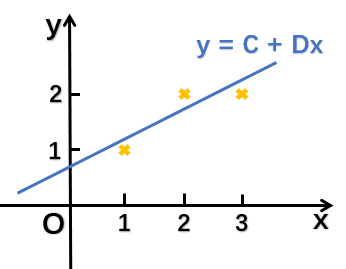
\includegraphics[scale=0.8]{figures/S16-1.png}
\end{center}
\begin{math}
	\left\{
	\begin{array}{rclrcl}
		C & + & D & = & 1 \\
		C & + & 2D & = & 2 \\
		C & + & 3D & = & 2 
	\end{array}
	\right.
\end{math}
 or 
\begin{math}
	\underbrace{
		\begin{bmatrix}
			1 & 1 \\
			1 & 2 \\
			1 & 3 
		\end{bmatrix}
	}_{\mathbf{A}}
	\underbrace{
		\begin{bmatrix}
			C \\
			D 
		\end{bmatrix}
	}_{\mathbf{x}}
	 = 
	\underbrace{
		\begin{bmatrix}
			1 \\
			2 \\
			2 
		\end{bmatrix}
	}_{\mathbf{b}}
\end{math}
\newline
${\mathbf{A}}{\mathbf{x}} = {\mathbf{b}}$ \qquad\qquad NO solution!
\newline
${\mathbf{A^{T}}}{\mathbf{A}}{\mathbf{\hat{x}}} = {\mathbf{A^{T}}}{\mathbf{b}}$ \qquad $\exists solution$!
\vspace{31pt}
\newline
复习一下 projection matrix 投影矩阵
\newline
${\mathbf{P}} = {\mathbf{A}}{\mathbf{({\mathbf{A^{T}}}{\mathbf{A}})^{-1}}} {\mathbf{A^{T}}}$
\newline
two extreme cases: 
\begin{itemize}
	\item if ${\mathbf{b}}$ is in column space of ${\mathbf{A}}$, then ${\mathbf{P}}{\mathbf{b}} = {\mathbf{b}}$
	\item if ${\mathbf{b}}$ is perpendicular to column space of ${\mathbf{A}}$ (${\mathbf{b}} \in N({\mathbf{A^{T}}})$), then ${\mathbf{P}}{\mathbf{b}} = {\mathbf{0}}$
\end{itemize}
usual cases:
\begin{center}
	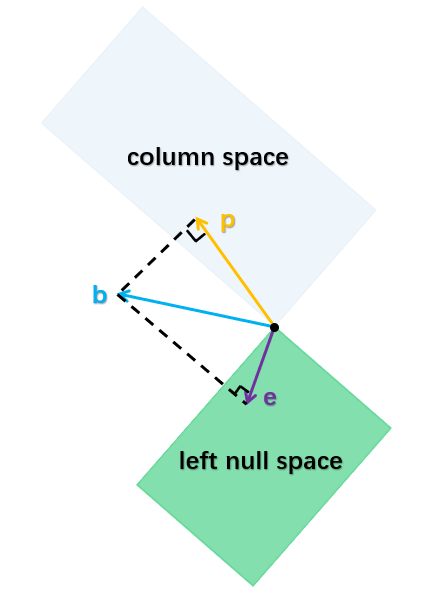
\includegraphics[scale=0.6]{figures/S16-2.png}
\end{center}
${\mathbf{p}} + {\mathbf{e}} = {\mathbf{b}}$ , where ${\mathbf{p}}$ is projection to $C({\mathbf{A}})$, ${\mathbf{e}}$ is projection to $N({\mathbf{A^{T}}})$
\newline
$\Longleftrightarrow$ ${\mathbf{P}}{\mathbf{b}}+({\mathbf{I}}-{\mathbf{P}}){\mathbf{b}} = {\mathbf{b}}$ , where $({\mathbf{I}}-{\mathbf{P}})$ is a projection matrix too, onto the perpendicular space
\vspace{31pt}
\newline
最小二乘,即最小平方和 \qquad $\min \quad {\text{error}}^2$
\begin{center}
	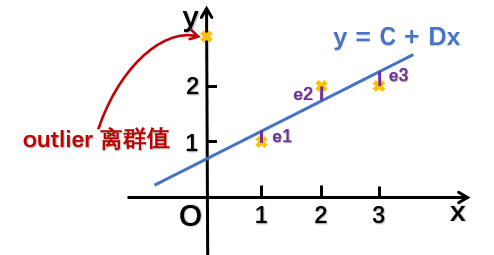
\includegraphics[scale=1.0]{figures/S16-3.png}
\end{center}
“最小二乘法很容易被离群值影响” so suppose no outliers!
\begin{displaymath}
	\min \quad e_1^2 + e_2^2 + e_3^2 = (C+D-1)^2 + (C+2D-2)^2 + (C+3D-2)^2
\end{displaymath}
to find 
\begin{math}
	\begin{bmatrix}
		\widehat{C} \\
		\widehat{D} 
	\end{bmatrix}
\end{math}
 = 
${\mathbf{\hat{x}}}$
, to solve 
\begin{math}
	{\mathbf{A^{T}}}{\mathbf{A}}{\mathbf{\hat{x}}} = 
	{\mathbf{A^{T}}}{\mathbf{A}}{
		\begin{bmatrix}
			\widehat{C} \\
			\widehat{D} 
		\end{bmatrix}
	} = 
	{\mathbf{A^{T}}}{\mathbf{b}}
\end{math}
\newline
then 
\begin{math}
	\left\{
	\begin{array}{rclrcl}
		3\widehat{C} & + & 6\widehat{D} & = & 5 \\
		6\widehat{C} & + & 14\widehat{D} & = & 11
	\end{array}
	\right.
	\quad 
	\Longrightarrow
	\left\{
	\begin{array}{rcl}
		\widehat{C} & = & \frac{2}{3} \\
		\widehat{D} & = & \frac{1}{2} 
	\end{array}
	\right.
	\quad 
	\Longrightarrow
	y=\cfrac{1}{2} x + \cfrac{2}{3}
\end{math}
\newline
suppose $p_1$, $p_2$, $p_3$ are the three values to substitute $b_1$, $b_2$, $b_3$
\newline
${\mathbf{b}} = {\mathbf{p}} + {\mathbf{e}}$ \quad i.e. \quad  
\begin{math}
	\begin{bmatrix}
		1 \\
		2 \\
		2 
	\end{bmatrix}
	 = 
	\begin{bmatrix}
		7/6 \\
		5/3 \\
		13/6 
	\end{bmatrix}
	 + 
	\begin{bmatrix}
		-1/6 \\
		1/3 \\
		-1/6 
	\end{bmatrix}
\end{math}
\newline
${\mathbf{p}} \perp {\mathbf{e}}$ ($\because$ ${\mathbf{p}} \in C({\mathbf{A}})$, ${\mathbf{e}} \in N({\mathbf{A^{T}}})$)
\vspace{31pt}
\newline
{\textcolor{anhao-scarlet}{fact: if ${\mathbf{A}}$ has independent columns, then ${\mathbf{A^{T}}}{\mathbf{A}}$ is invertible}}
\newline
proof:
\par suppose ${\mathbf{A^{T}}}{\mathbf{A}}{\mathbf{x}} = {\mathbf{0}}$, to prove ${\mathbf{x}}$ must be ${\mathbf{0}}$
\par (trick) ${\mathbf{x^{T}}}{\mathbf{A^{T}}}{\mathbf{A}}{\mathbf{x}} = {\mathbf{0}}$
\par $\Longrightarrow$ $({\mathbf{Ax}})^{\mathbf{T}}{\mathbf{Ax}} = {\mathbf{0}}$
\par $\xrightarrow{{\mathbf{y}}={\mathbf{Ax}} {\text{, is a col vector}}}$ ${\mathbf{y^{T}}}{\mathbf{y}} = {\mathbf{0}}$
\par $\Longleftrightarrow$ ${\mathbf{y}} = {\mathbf{0}}$
\par $\therefore$ ${\mathbf{Ax}}$ has to be ${\mathbf{0}}$
\par to use the hypothesis: ${\mathbf{A}}$ has independent columns
\par ${\mathbf{x}}$ has to be ${\mathbf{0}}$

\newpage
\section{Lecture 17 - 正交矩阵、格拉姆-施密特正交化}
\pagestyle{fancy}
\lhead{}
\chead{Lecture 17 - 正交矩阵、格拉姆-施密特正交化}
\rhead{}

\noindent 有一种特别的线性无关:
columns are definitely independent if they are perpendicular unit vectors, i.e. orthogonal-normal vectors, or orthonormal vectors in short
\vspace{14pt}
\newline
orthonormal basis ${\mathbf{q_1}}$, ${\mathbf{q_2}}$, $\cdots$, ${\mathbf{q_n}}$ \quad such that \quad 
\begin{math}
	{\mathbf{q_i^T}}{\mathbf{q_j}} = 
	\begin{cases}
		0,  & \text{if $i \neq j$} \\
		1,  & \text{if $i = j$}
	\end{cases}
\end{math}
\vspace{14pt}
\newline
How does having an orthonormal basis make things better? "they never overflow or underflow"\footnote{{\ding{73}}意{\ding{73}}義{\ding{73}}不{\ding{73}}明{\ding{73}}}
\vspace{31pt}
\newline
orthonormal matrix ${\mathbf{Q}}$ (square)
\newline
\begin{math}
	{\mathbf{Q}} = 
	\begin{bmatrix}
		\ & | & \ & \ & \ & | & \ \\
		\ & {\mathbf{q_1}} & \ & \cdots & \ & {\mathbf{q_n}} & \ \\
		\ & | & \ & \ & \ & | & \ 
	\end{bmatrix}
\end{math}
\newline
\begin{math}
	{\mathbf{Q^{T}}}{\mathbf{Q}} = 
	\begin{bmatrix}
		-- & {\mathbf{q_1^T}} & -- \\
		\ & \ & \ \\
		\ & \vdots & \ \\
		\ & \ & \ \\
		-- & {\mathbf{q_n^T}} & -- 
	\end{bmatrix}
	\begin{bmatrix}
		\ & | & \ & \ & \ & | & \ \\
		\ & {\mathbf{q_1}} & \ & \cdots & \ & {\mathbf{q_n}} & \ \\
		\ & | & \ & \ & \ & | & \ 
	\end{bmatrix}
	 = 
	\begin{bmatrix}
		1 & 0 & \cdots & 0 \\
		0 & 1 & \cdots & 0 \\
		\vdots & \vdots & \ddots & \vdots \\
		0 & 0 & \cdots & 1 \\
	\end{bmatrix}
	 = 
	{\mathbf{I}}
\end{math}
\newline
if ${\mathbf{Q}}$ is square, then ${\mathbf{Q^{T}}}{\mathbf{Q}} = {\mathbf{I}}$ tells that ${\mathbf{Q^{T}}} = {\mathbf{Q^{-1}}}$
\newline
{\textcolor{anhao-scarlet}{注:若 ${\mathbf{Q}}$ 不是方阵,则未必有 ${\mathbf{Q}}{\mathbf{Q^{T}}} = {\mathbf{I}}$ ,但仍然有 ${\mathbf{Q^{T}}}{\mathbf{Q}} = {\mathbf{I}}$ !}}
\vspace{31pt}
\newline
in case that the columns of ${\mathbf{A}}$ are not orthonormal, how can I make them so?
\newline
{\textcolor{anhao-scarlet}{Graham-Schmidt}}
\par to start with independent vectors, and we want to make "them"\footnote{not original ones} orthonormal
\newline
{\textcolor{anhao-scarlet}{思想:原来的 ${\mathbf{A}}$ 的各列张成(span)一个列空间 $C({\mathbf{A}})$ ,${\mathbf{A}}$ 的列是 $C({\mathbf{A}})$ 的一组基,但这组基还不够好(不正交)。现在通过 Graham-Schmidt 方法去找 $C({\mathbf{A}})$ 的一组标准正交基。}}
\vspace{31pt}
\newline
what's the good of having a ${\mathbf{Q}}$? what formulas become easier?
\newline
suppose ${\mathbf{Q}}$ has orthonormal columns, to project onto its column space, 
\par 
\begin{math}
	{\mathbf{P}} = {\mathbf{Q}}({\mathbf{Q^{T}}}{\mathbf{Q}})^{\mathbf{-1}}{\mathbf{Q^{T}}} = 
	{\mathbf{Q}}\cdot{\mathbf{I}}\cdot{\mathbf{Q^{T}}} = 
	{\mathbf{Q}}{\mathbf{Q^{T}}} 
	\quad ( = {\mathbf{I}} \ {\text{if}} \ {\mathbf{Q}} \ {\text{is square}} )
\end{math}
\par 
\begin{math}
	({\mathbf{Q}}{\mathbf{Q^{T}}})({\mathbf{Q}}{\mathbf{Q^{T}}}) = {\mathbf{Q}}{\mathbf{Q^{T}}}
\end{math}
\newline
to solve the normal equations,
\par ${\mathbf{A^{T}}}{\mathbf{A}}{\mathbf{\hat{x}}} = {\mathbf{A^{T}}}{\mathbf{b}}$
\par now ${\mathbf{A}}$ is ${\mathbf{Q}}$,
\par ${\mathbf{Q^{T}}}{\mathbf{Q}}{\mathbf{\hat{x}}} = {\mathbf{Q^{T}}}{\mathbf{b}}$ $\Longleftrightarrow$ ${\mathbf{\hat{x}}} = {\mathbf{Q^{T}}}{\mathbf{b}}$
\vspace{31pt}
\newline
二维的情形:
\newline
independent vectors ${\mathbf{a}}$, ${\mathbf{b}}$ $\longrightarrow$ orthogonal vectors ${\mathbf{A}}$, ${\mathbf{B}}$ $\longrightarrow$ orthonormal vectors $\cfrac{\mathbf{A}}{\Vert{\mathbf{A}}\Vert}$, $\cfrac{\mathbf{B}}{\Vert{\mathbf{B}}\Vert}$
\begin{center}
	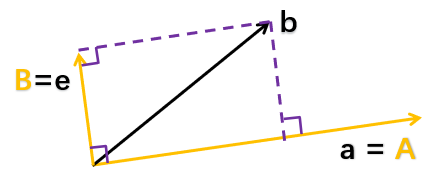
\includegraphics[scale=0.8]{figures/S17-1.png}
\end{center}
\begin{math}
	{\mathbf{B}} = {\mathbf{b}} - \cfrac{{\mathbf{A}}{\mathbf{A^{T}}}}{{\mathbf{A^{T}}}{\mathbf{A}}}{\mathbf{b}} = {\mathbf{e}}
\end{math}
\qquad then ${\mathbf{B}} \perp {\mathbf{A}}$
\vspace{14pt}
\newline
三维的情形:
\newline
independent vectors ${\mathbf{a}}$, ${\mathbf{b}}$, ${\mathbf{c}}$
\par\quad $\longrightarrow$ orthogonal vectors ${\mathbf{A}}$, ${\mathbf{B}}$, ${\mathbf{C}}$
\par\qquad\qquad $\longrightarrow$ orthonormal vectors $\cfrac{\mathbf{A}}{\Vert{\mathbf{A}}\Vert}$, $\cfrac{\mathbf{B}}{\Vert{\mathbf{B}}\Vert}$, $\cfrac{\mathbf{C}}{\Vert{\mathbf{C}}\Vert}$
\newline
idea: ${\mathbf{C}}$ 向 ${\mathbf{A}}$、${\mathbf{B}}$ 所张成的平面投影
\newline
\begin{math}
	{\mathbf{C}} = {\mathbf{c}} - \cfrac{{\mathbf{A}}{\mathbf{A^{T}}}}{{\mathbf{A^{T}}}{\mathbf{A}}}{\mathbf{c}} - \cfrac{{\mathbf{B}}{\mathbf{B^{T}}}}{{\mathbf{B^{T}}}{\mathbf{B}}}{\mathbf{c}}
\end{math}
\qquad then ${\mathbf{C}} \perp {\mathbf{A}}$ and ${\mathbf{C}} \perp {\mathbf{B}}$
\vspace{31pt}
\newline
example: 
\begin{math}
	{\mathbf{a}} = 
	\begin{bmatrix}
		1 \\
		1 \\
		1 
	\end{bmatrix}
\end{math}
, 
\begin{math}
	{\mathbf{b}} = 
	\begin{bmatrix}
		1 \\
		0 \\
		2 
	\end{bmatrix}
\end{math}
\begin{math}
	\left(
	{\mathbf{T}} = 
	\begin{bmatrix}
		\ | & | \ \\
		\ {\mathbf{a}} & {\mathbf{b}} \ \\
		\ | & | \ 
	\end{bmatrix}
	 = 
	\begin{bmatrix}
		1 & 1 \\
		1 & 0 \\
		1 & 2 
	\end{bmatrix}
	\right)
\end{math}
\newline
solution:
\par 
\begin{math}
	{\mathbf{A}} = {\mathbf{a}} = 
	\begin{bmatrix}
		1 \\
		1 \\
		1 
	\end{bmatrix}
\end{math}
\par 
\begin{math}
	{\mathbf{B}} = 
	\begin{bmatrix}
		1 \\
		0 \\
		2 
	\end{bmatrix}
	 - 
	\cfrac{
		\begin{bmatrix}
			1 & 1 & 1 \\
			1 & 1 & 1 \\
			1 & 1 & 1 
		\end{bmatrix}
	}
	{
		\begin{bmatrix}
			1 & 1 & 1 
		\end{bmatrix}
		\begin{bmatrix}
			1 \\
			1 \\
			1 
		\end{bmatrix}
	}
	\begin{bmatrix}
		1 \\
		0 \\
		2 
	\end{bmatrix}
	 = 
	\begin{bmatrix}
		1 \\
		0 \\
		2 
	\end{bmatrix}
	 - 
	\begin{bmatrix}
		1 \\
		1 \\
		1 
	\end{bmatrix}
	 = 
	\begin{bmatrix}
		0 \\
		-1 \\
		1 
	\end{bmatrix}
\end{math}
\par check: ${\mathbf{A}} \perp {\mathbf{B}}$
\par
\begin{math}
	{\mathbf{q_1}} = 
	\begin{bmatrix}
		\cfrac{1}{\sqrt{3}} \\
		\cfrac{1}{\sqrt{3}} \\
		\cfrac{1}{\sqrt{3}} 
	\end{bmatrix}
\end{math}
, 
\begin{math}
	{\mathbf{q_2}} = 
	\begin{bmatrix}
		0 \\
		-\cfrac{1}{\sqrt{2}} \\
		\cfrac{1}{\sqrt{2}} 
	\end{bmatrix}
\end{math}
\par 
\begin{math}
	{\mathbf{Q}} = 
	\begin{bmatrix}
		\ | & | \ \\
		\ {\mathbf{q_1}} & {\mathbf{q_2}} \ \\
		\ | & | \ 
	\end{bmatrix}
	 = 
	\begin{bmatrix}
		\cfrac{1}{\sqrt{3}} & 0 \\
		\cfrac{1}{\sqrt{3}} & -\cfrac{1}{\sqrt{2}} \\
		\cfrac{1}{\sqrt{3}} & \cfrac{1}{\sqrt{2}} 
	\end{bmatrix}
\end{math}
\vspace{14pt}
\par {\textcolor{anhao-scarlet}{the fact: $C({\mathbf{Q}}) = C({{\mathbf{T}}})$ !}}
\vspace{14pt}
\par 
\begin{math}
	\begin{bmatrix}
		\ | & | \ \\
		\ {\mathbf{a}} & {\mathbf{b}} \ \\
		\ | & | \ 
	\end{bmatrix}
	 = 
	\begin{bmatrix}
		\ | & | \ \\
		\ {\mathbf{q_1}} & {\mathbf{q_2}} \ \\
		\ | & | \ 
	\end{bmatrix}
	\begin{bmatrix}
		{\mathbf{q_1^T}}{\mathbf{a}} & {\mathbf{q_1^T}}{\mathbf{b}} \\
		{\mathbf{q_2^T}}{\mathbf{a}} & {\mathbf{q_2^T}}{\mathbf{b}}
	\end{bmatrix}
	 = 
	\begin{bmatrix}
		\ | & | \ \\
		\ {\mathbf{q_1}} & {\mathbf{q_2}} \ \\
		\ | & | \ 
	\end{bmatrix}
	\begin{bmatrix}
		{\mathbf{q_1^T}}{\mathbf{a}} & {\mathbf{q_1^T}}{\mathbf{b}} \\
		0 & {\mathbf{q_2^T}}{\mathbf{b}}
	\end{bmatrix}
\end{math}
\par 可以直接看出 ${\mathbf{a}}$ 与 ${\mathbf{b}}$ 分别在 $\left\{{\mathbf{q_1}}, {\mathbf{q_2}}\right\}$ 坐标系中的坐标为 $({\mathbf{q_1^T}}{\mathbf{a}}, 0)$ 与 $({\mathbf{q_1^T}}{\mathbf{b}}, {\mathbf{q_2^T}}{\mathbf{b}})$ 。

\end{document}